\documentclass{ltjsbook}
\usepackage{docmute} 
\usepackage{../../myStyle} 

\begin{document}
\chapter{Inference and Judgement}
\label{m17_estimation_and_test}
Last time, we talked about a method called "method of moments" to estimate population parameters using descriptive statistics of a sample.
Now, let's continue with this story and talk about how to estimate the population parameters, using the normal distribution, which is commonly used in psychology, as an example.
As a purpose of psychology, it is sometimes more important to consider relative comparisons rather than the actual numerical values of the variables. This way of thinking leads to the discussion of model comparisons. It is important to note that the TeX code should not be altered.

\section{Unbiased Estimators}
In the previous discussion, we saw that the sample mean converges to the population mean and we can also determine the variability. Therefore, it seems possible to estimate the population from the sample. Although the sample mean may contain some deviation, it can be used as an estimate for the population mean. For instance, using the example of the heights of three students, we can make a prediction that the population mean might be around 173cm. Of course, due to the small sample size, there may still be some deviation of around $\pm$ a few centimeters.

By the way, when we insist on a specific value for the estimate of the population mean and say "The estimated value of the population mean is XXX!" it is called \textit{point estimation}. However, this is quite a gamble since it is unlikely that we will hit the exact answer (population mean) spot on, even though we may get close to it. In particular, for continuous variables, it is unlikely that the estimate will match the exact value down to several decimal places. To account for this, we can predict a "range of deviation" in our estimate. This is known as \textit{interval estimation}. Instead of insisting that the population mean is exactly 173cm, we predict that it falls within the range of 160cm to 180cm. This way, the likelihood of our estimate being off is reduced. However, insisting that the value is between 0cm and 500cm does not actually provide any estimate at all. Therefore, we need to consider the width and probability of the range such as that there is a 95\% probability that the interval is within 5cm of 173cm.

This indirect and slightly cautious method of estimation seems to be working well, but there are still some issues remaining. In order to express this range, we need to estimate how much the sample mean varies and the width of that variation. Yes, we need the standard error. However, since the variance of the sample mean (the standard error) depends on the population variance, we must consider what the population variance is.

One idea for estimating the population variance is to use the sample variance, just like we used the sample mean as an estimate for the population mean. However, unfortunately, this method does not work well as shown in Figure \ref{fig::16_5}.
\begin{figure}[ht]
    \centering
    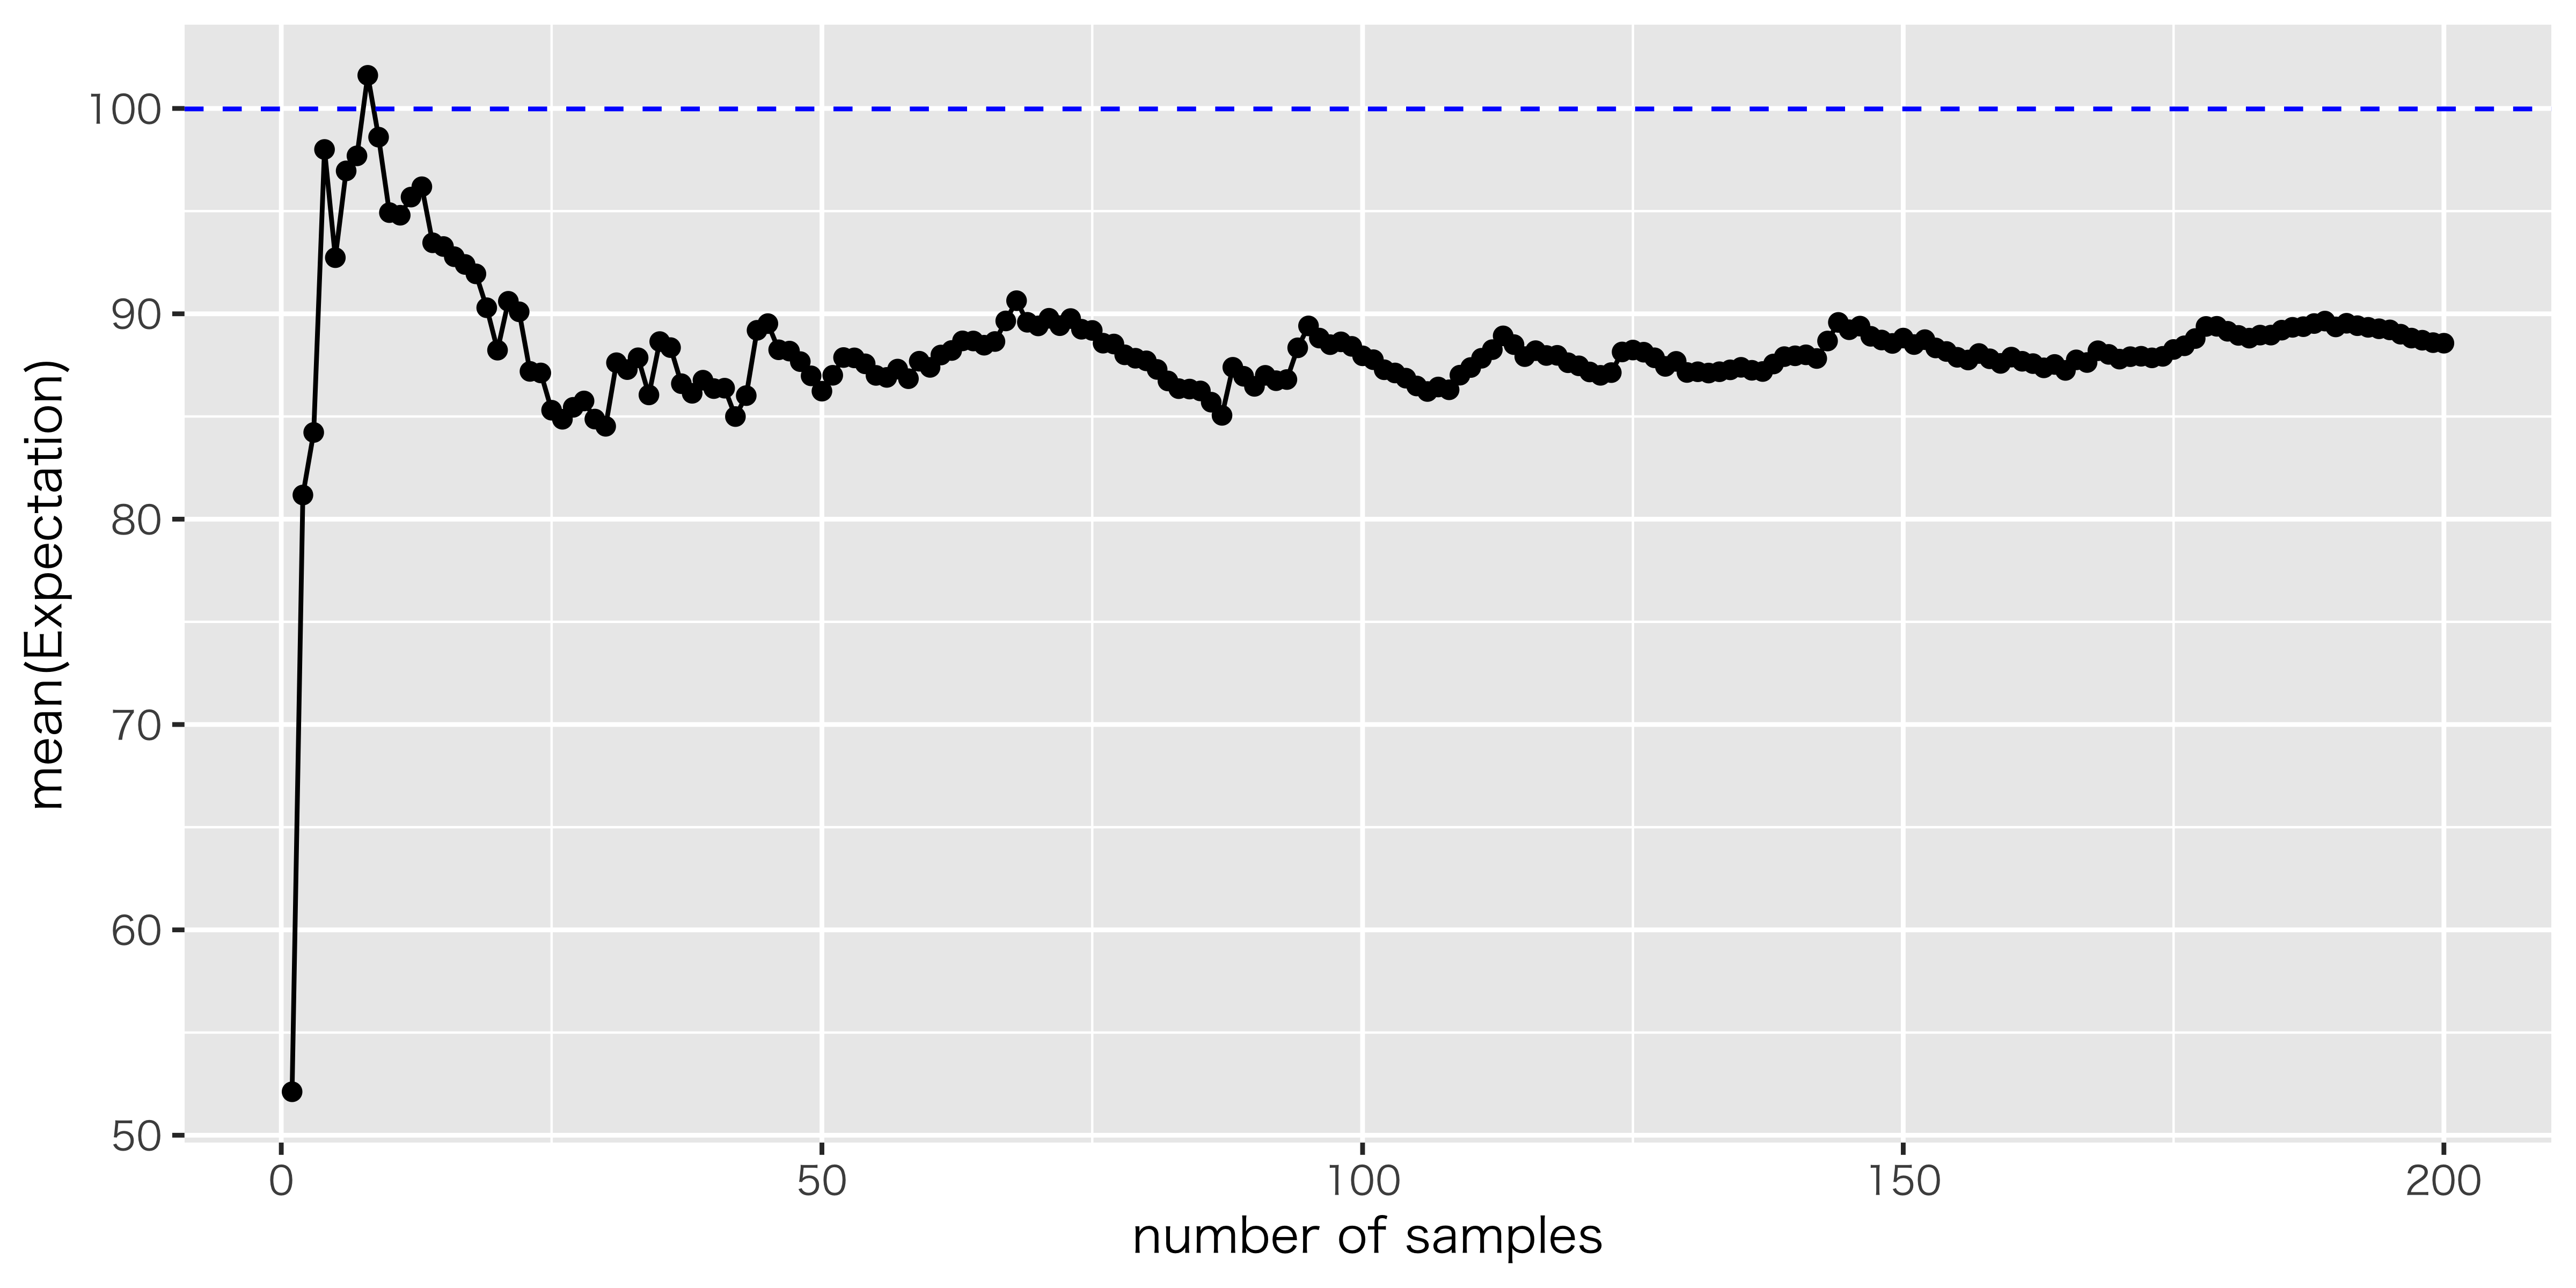
\includegraphics[keepaspectratio,height=0.4\linewidth]{../images/16_inference/Rplot16_04.png}
    \caption{By repeating the sampling and calculating the average of the sample variance, it deviates slightly from the population variance.}
    \label{fig::16_5}
\end{figure}

This is the result obtained by repeatedly sampling 10 samples 200 times, just like when obtaining the sample mean, and sequentially taking the average of the sample variances. Looking at this... Oh, it seems to be converging to the lower side of the blue line representing the true value (population variance). This deviation is called bias. While the sample mean is an unbiased estimator, the variance has bias.

In fact, it is known that the expected value (mean) of the sample variance does not equal the population variance. However, it seems that the magnitude of this difference is constant. In fact, it is computable (without delving into the details of mathematical statistics) that the magnitude of the difference is $\frac{\sigma^2}{n}$.

If you know the degree of deviation, you can plan the calculation from the beginning to match the calculation. Do you remember the formula for calculating sample variance? It was a formula like this.
\begin{equation}
	s_X^2=\frac{1}{n}\sum(X_i - \bar{X})^2
\end{equation}

If this is the expected value of the sample distribution,\footnote{The expected value of a probability distribution is the average value of the random variable. If you have forgotten this, please refer to Section \ref{expectation}, Pp. \pageref{expectation}.} and it is off from the population variance by $\frac{\sigma^2}{n}$, we would like to consider this deviation in advance in order to estimate the population variance $\sigma^2$. Let us expand the equation.
No Japanese words are present in the given TeX code.

This calculation will be done beforehand as an estimated value.
The equation contains only mathematical symbols and not Japanese words, therefore no translation is necessary.

So, I was able to correct it in advance to prevent this shift from happening.

The variance (sample variance) as a descriptive statistic is divided by the sample size $n$, while the estimated variance $\hat{\sigma^2}$ as an inferential statistic is divided by a slightly smaller value, $n-1$. This is known as an unbiased sample statistic, and is called the unbiased variance.

Using the formula for unbiased variance, the simulation from earlier was conducted and is shown in figure \ref{fig::16_6}. As you can see, the corrected unbiased variance is getting closer to the population variance.
\begin{figure}[ht]
	\centering
	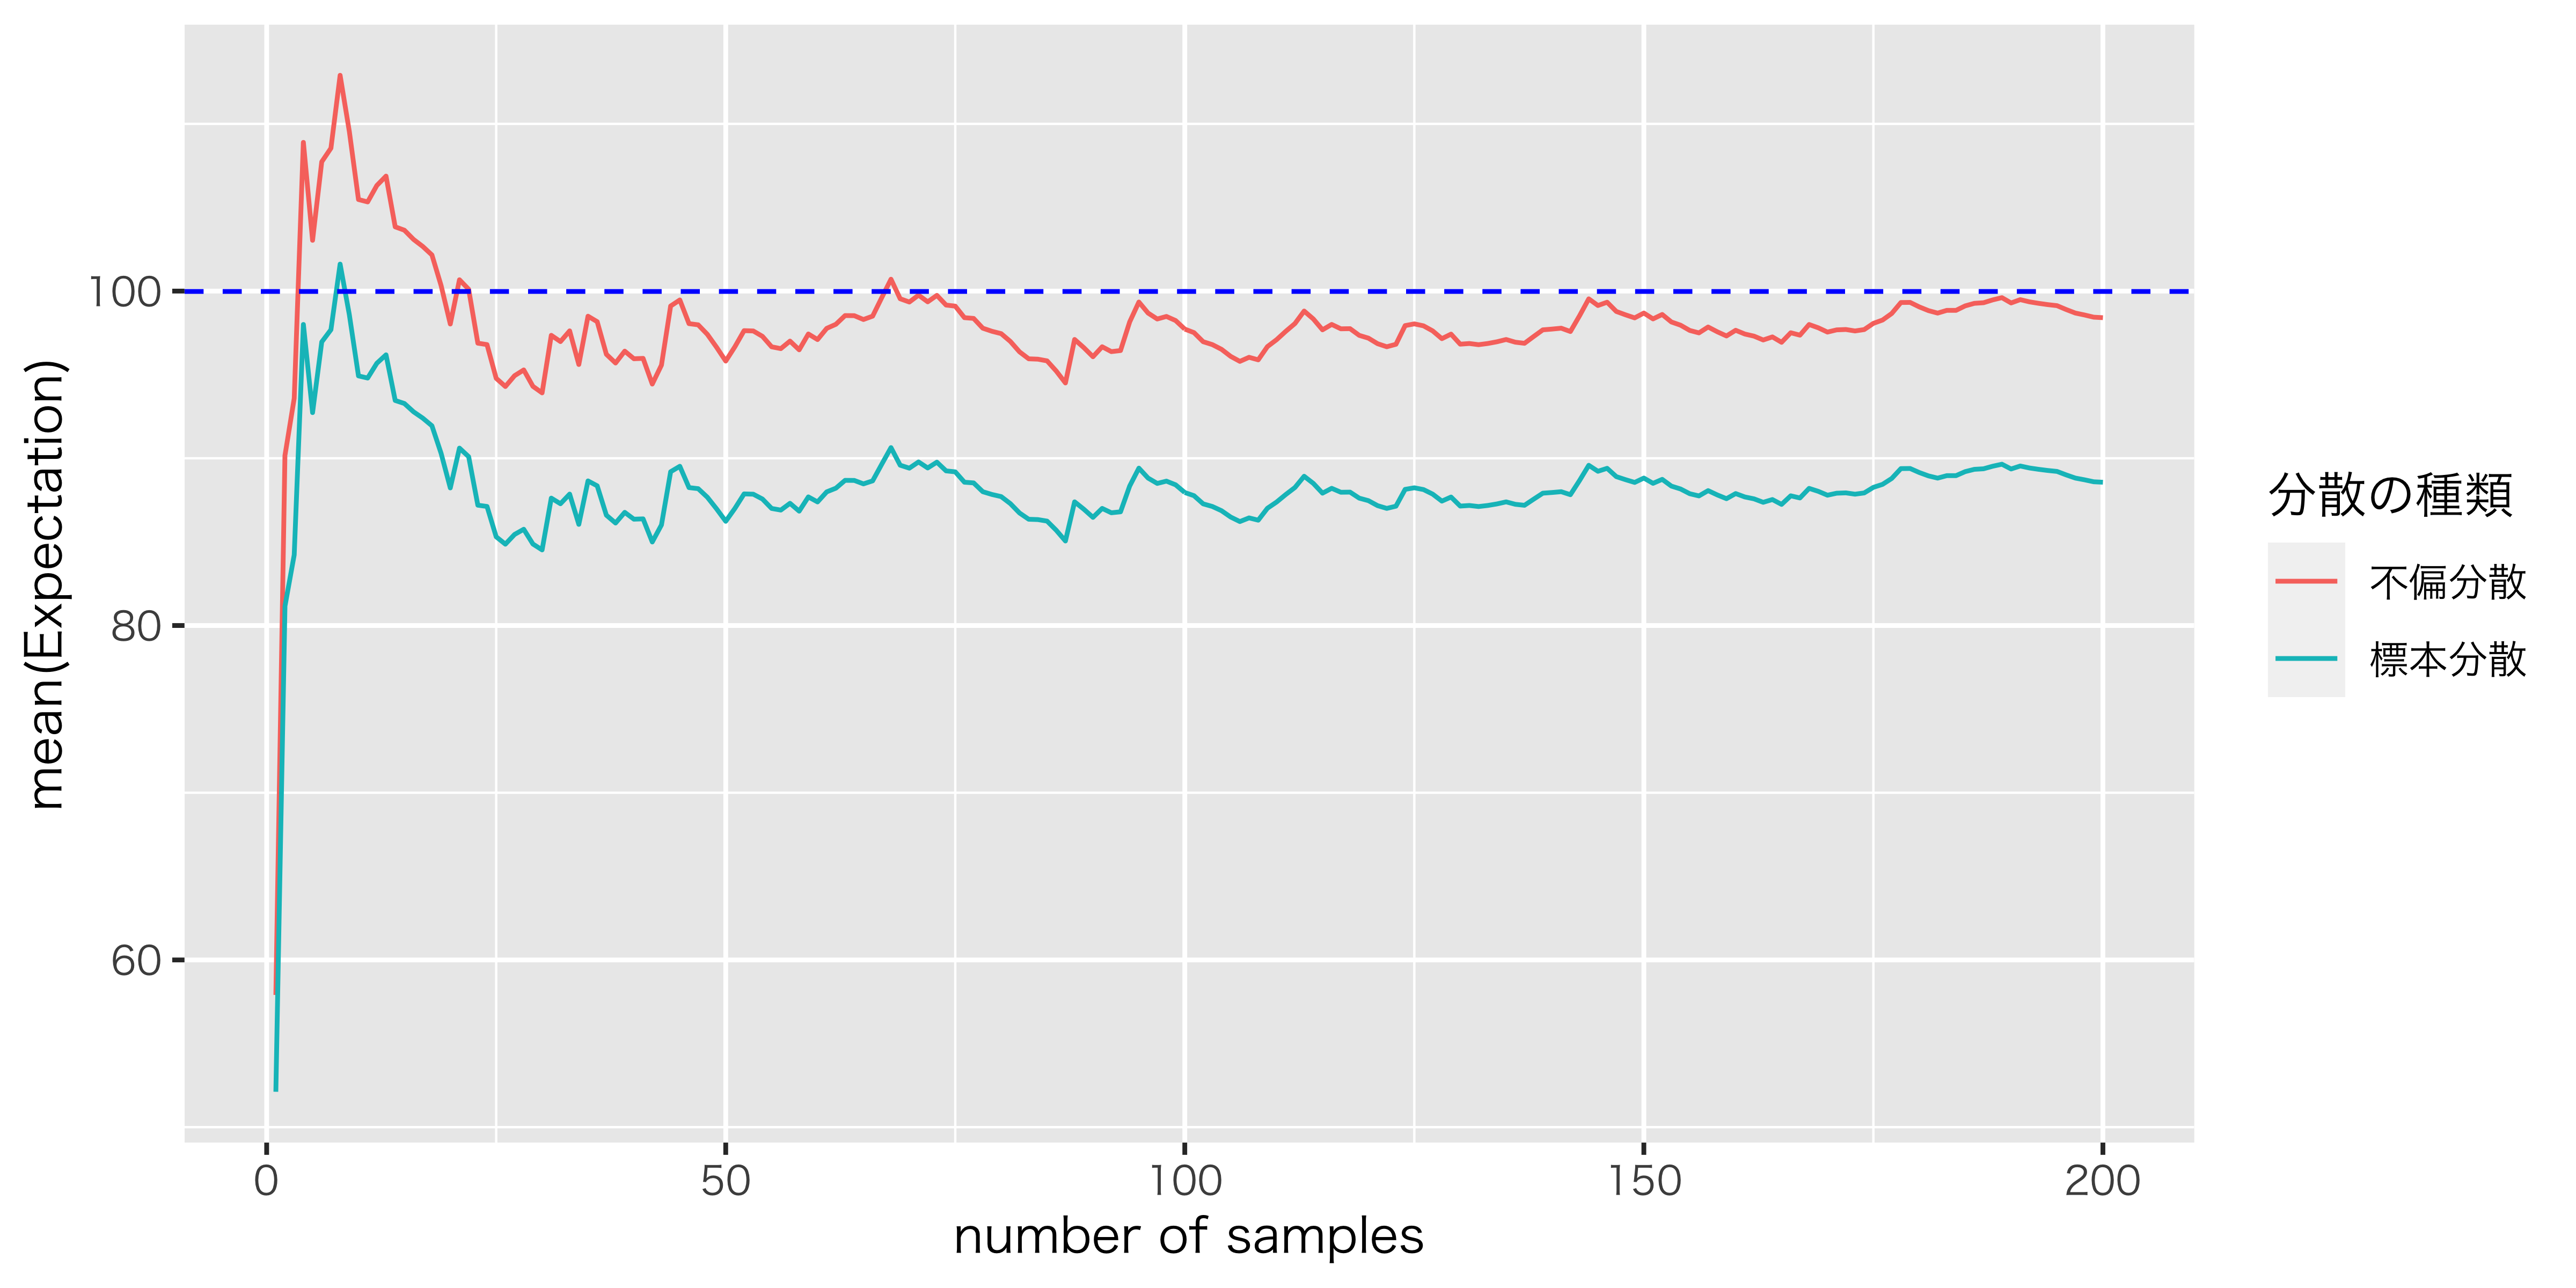
\includegraphics[keepaspectratio,height=0.4\linewidth]{../images/16_inference/Rplot16_05.png}
	\caption{サンプリングを繰り返し，標本分散と不偏分散の期待値を求めたもの}
	\label{fig::16_6}
\end{figure}



\section{Interval Estimation for Sample Means}
Previously, we discussed estimation using the normal distribution (refer to Section \ref{UsefulNormal}, p. \pageref{UsefulNormal}). Let's revisit that discussion.
Let's say a score $x$ follows a normal distribution, which is expressed as follows.\footnote{The normal distribution is also known as the Normal Curve and can be abbreviated as N. It has two parameters: the mean and standard deviation. Some statistics textbooks may refer to mean and variance instead, since the variance is the squared deviation of the standard deviation ($\to$ Lecture \ref{m05_descriptives}). However, this is just a matter of notation, as both provide the same information. In this book, we use the standard deviation in line with the notation in the statistical environment R.}
\[ x\sim N(\mu,\sigma) \]
If you standardize the variable $x$, it will follow the standard normal distribution. In other words, ...
\begin{figure}[ht]
    \centering
    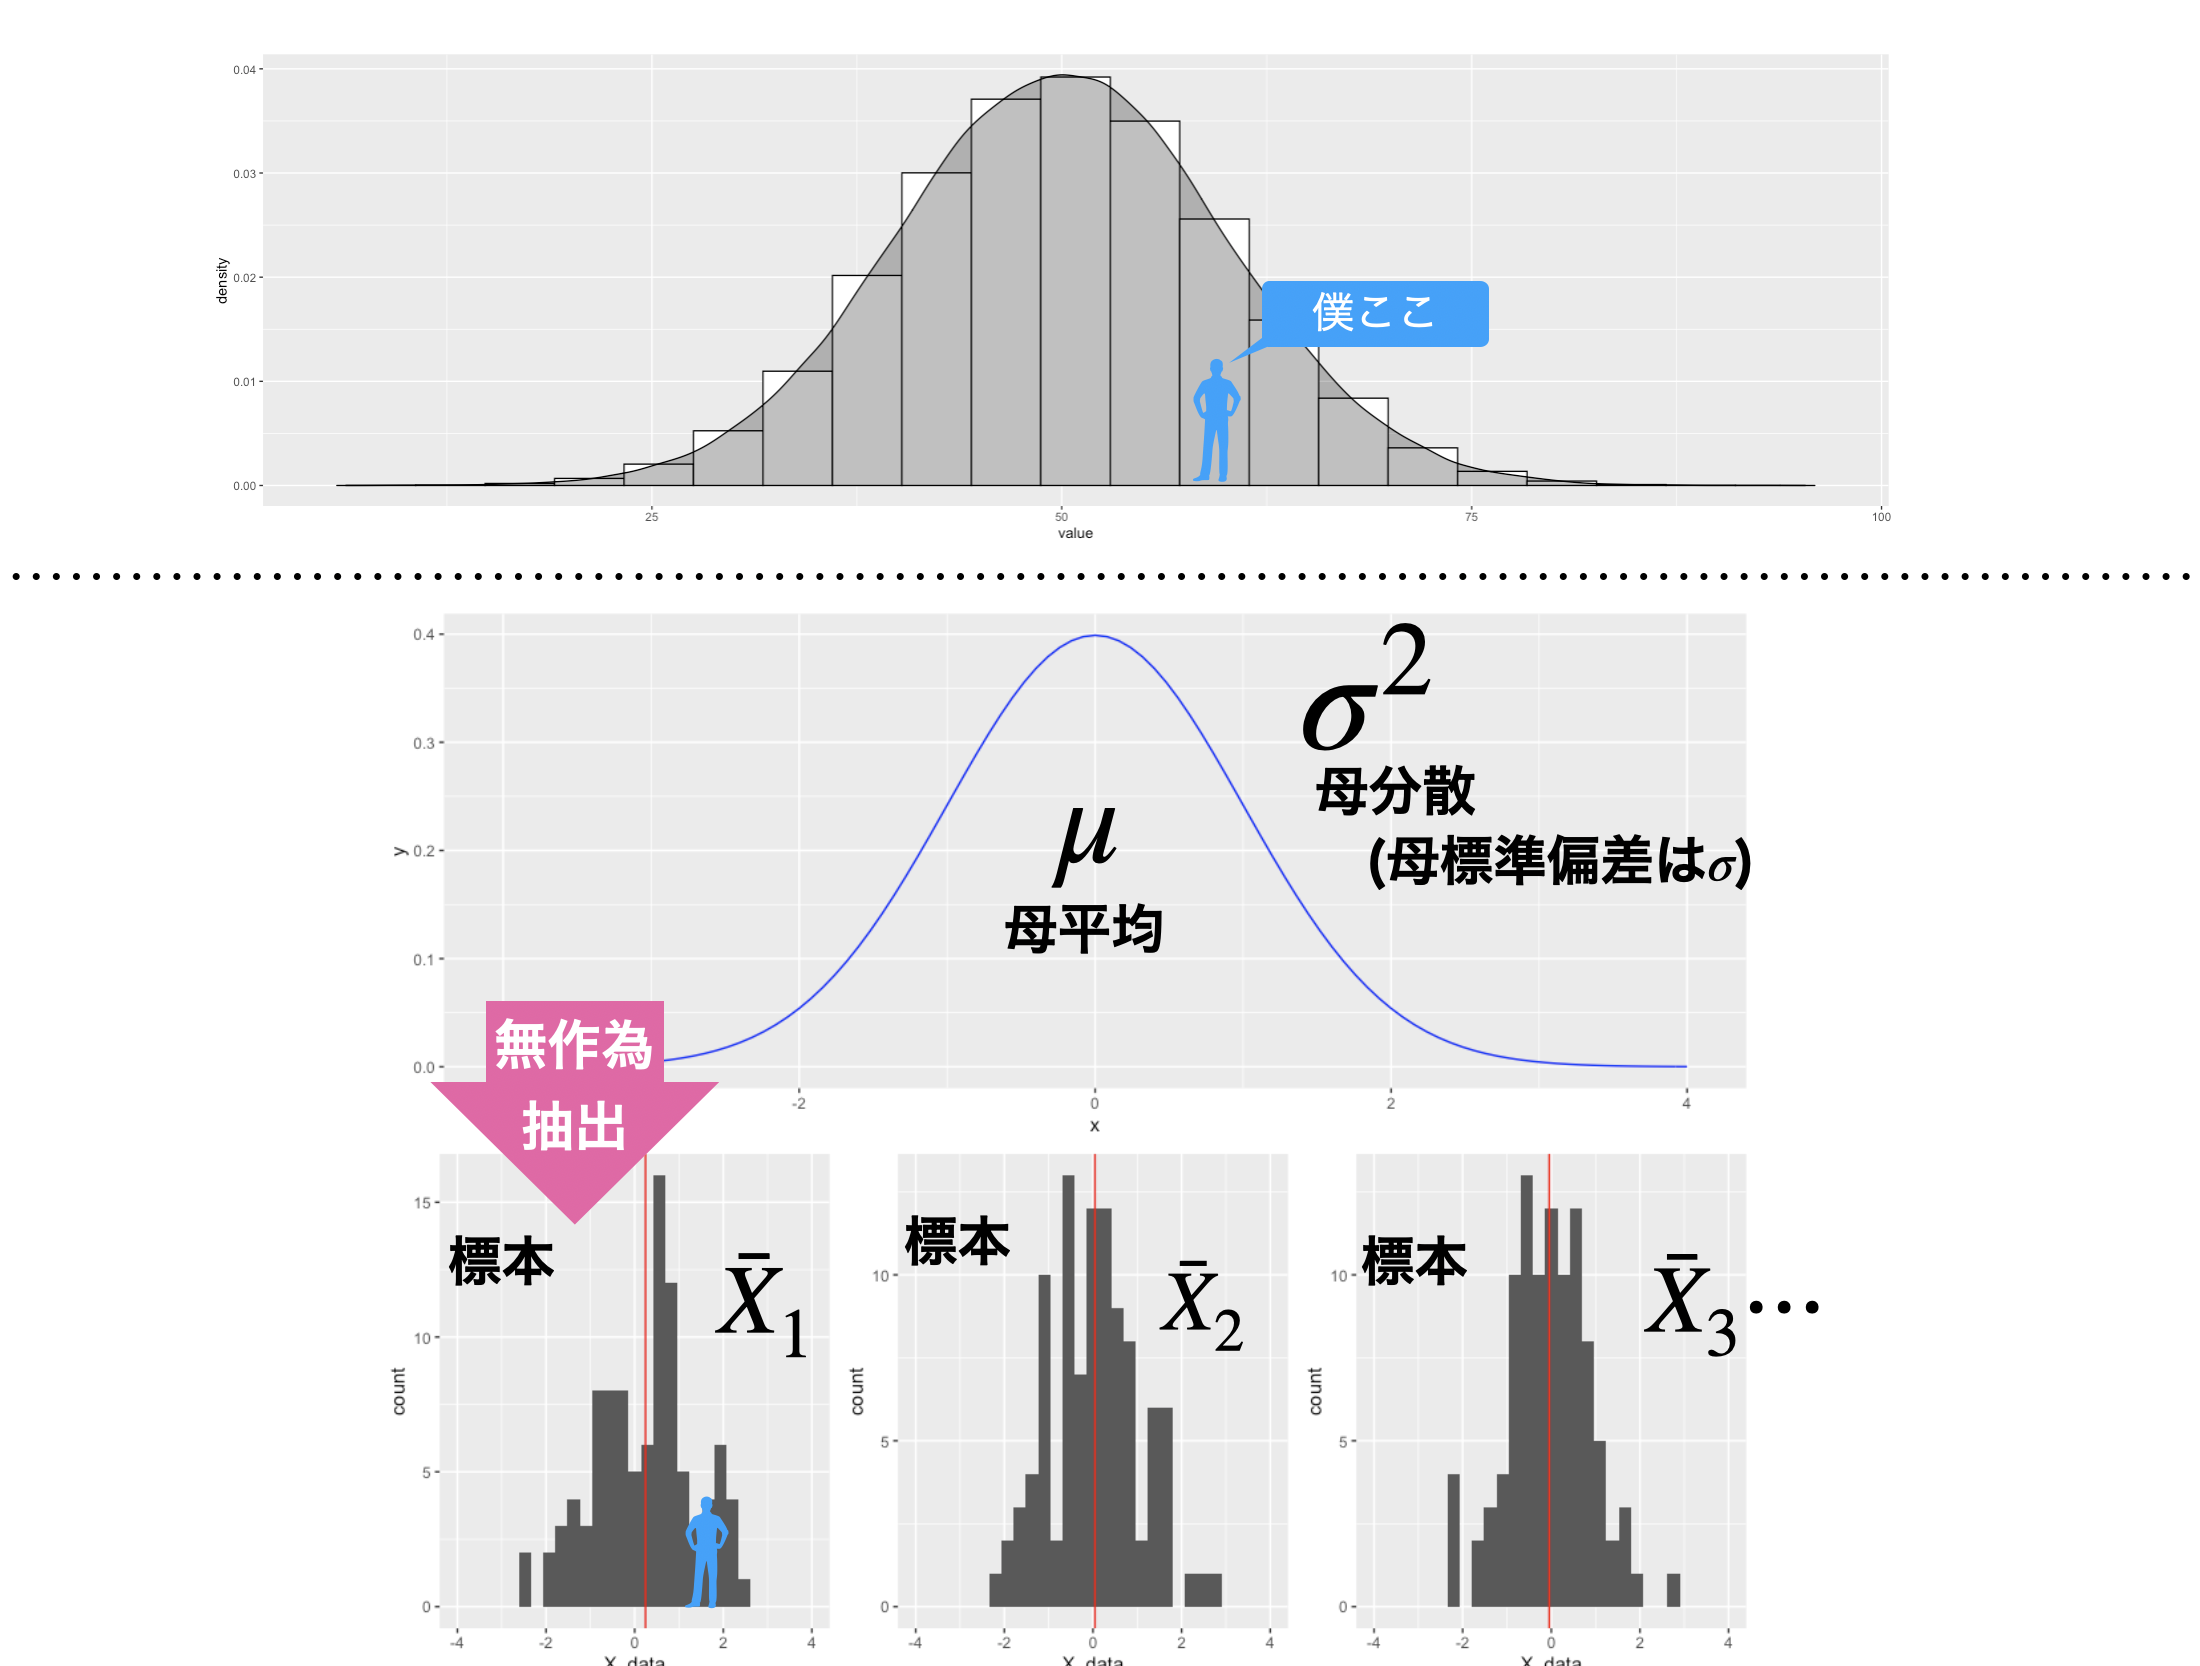
\includegraphics[keepaspectratio,height=0.6\linewidth]{../images/17_estimation_and_test/slide17_1.png}
    \caption{推測統計学の枠組みで考えることに注意。以前(セクション\ref{UsefulNormal})は上の図のように，推測するのではなくて母集団そのものの中に一個人のスコアを位置付けて，相対的な位置を考えよう，という話でした。今回は下のように，母集団が正規分布だと仮定して，そこから得られた標本のことについて考えています。個々のデータは標本の中にあります。また今回考えるのは標本統計量で，それが標本分布に従うのでした。}
    \label{fig::17_01}
\end{figure}

\[ z \sim N(0,1) \]
So the point was that by referring to tables of the standard normal distribution, one can estimate relative positions.

I would like to reconsider this within the framework of population and sample (see Figure \ref{fig::17_01}). The previous discussion started with the assumption that a score follows a normal distribution with mean $\mu$ and standard deviation $\sigma$, which is denoted by Greek letters and referred to as population parameters. It would be easy if we knew the population parameters in advance.

\begin{figure}[ht]
    \centering
    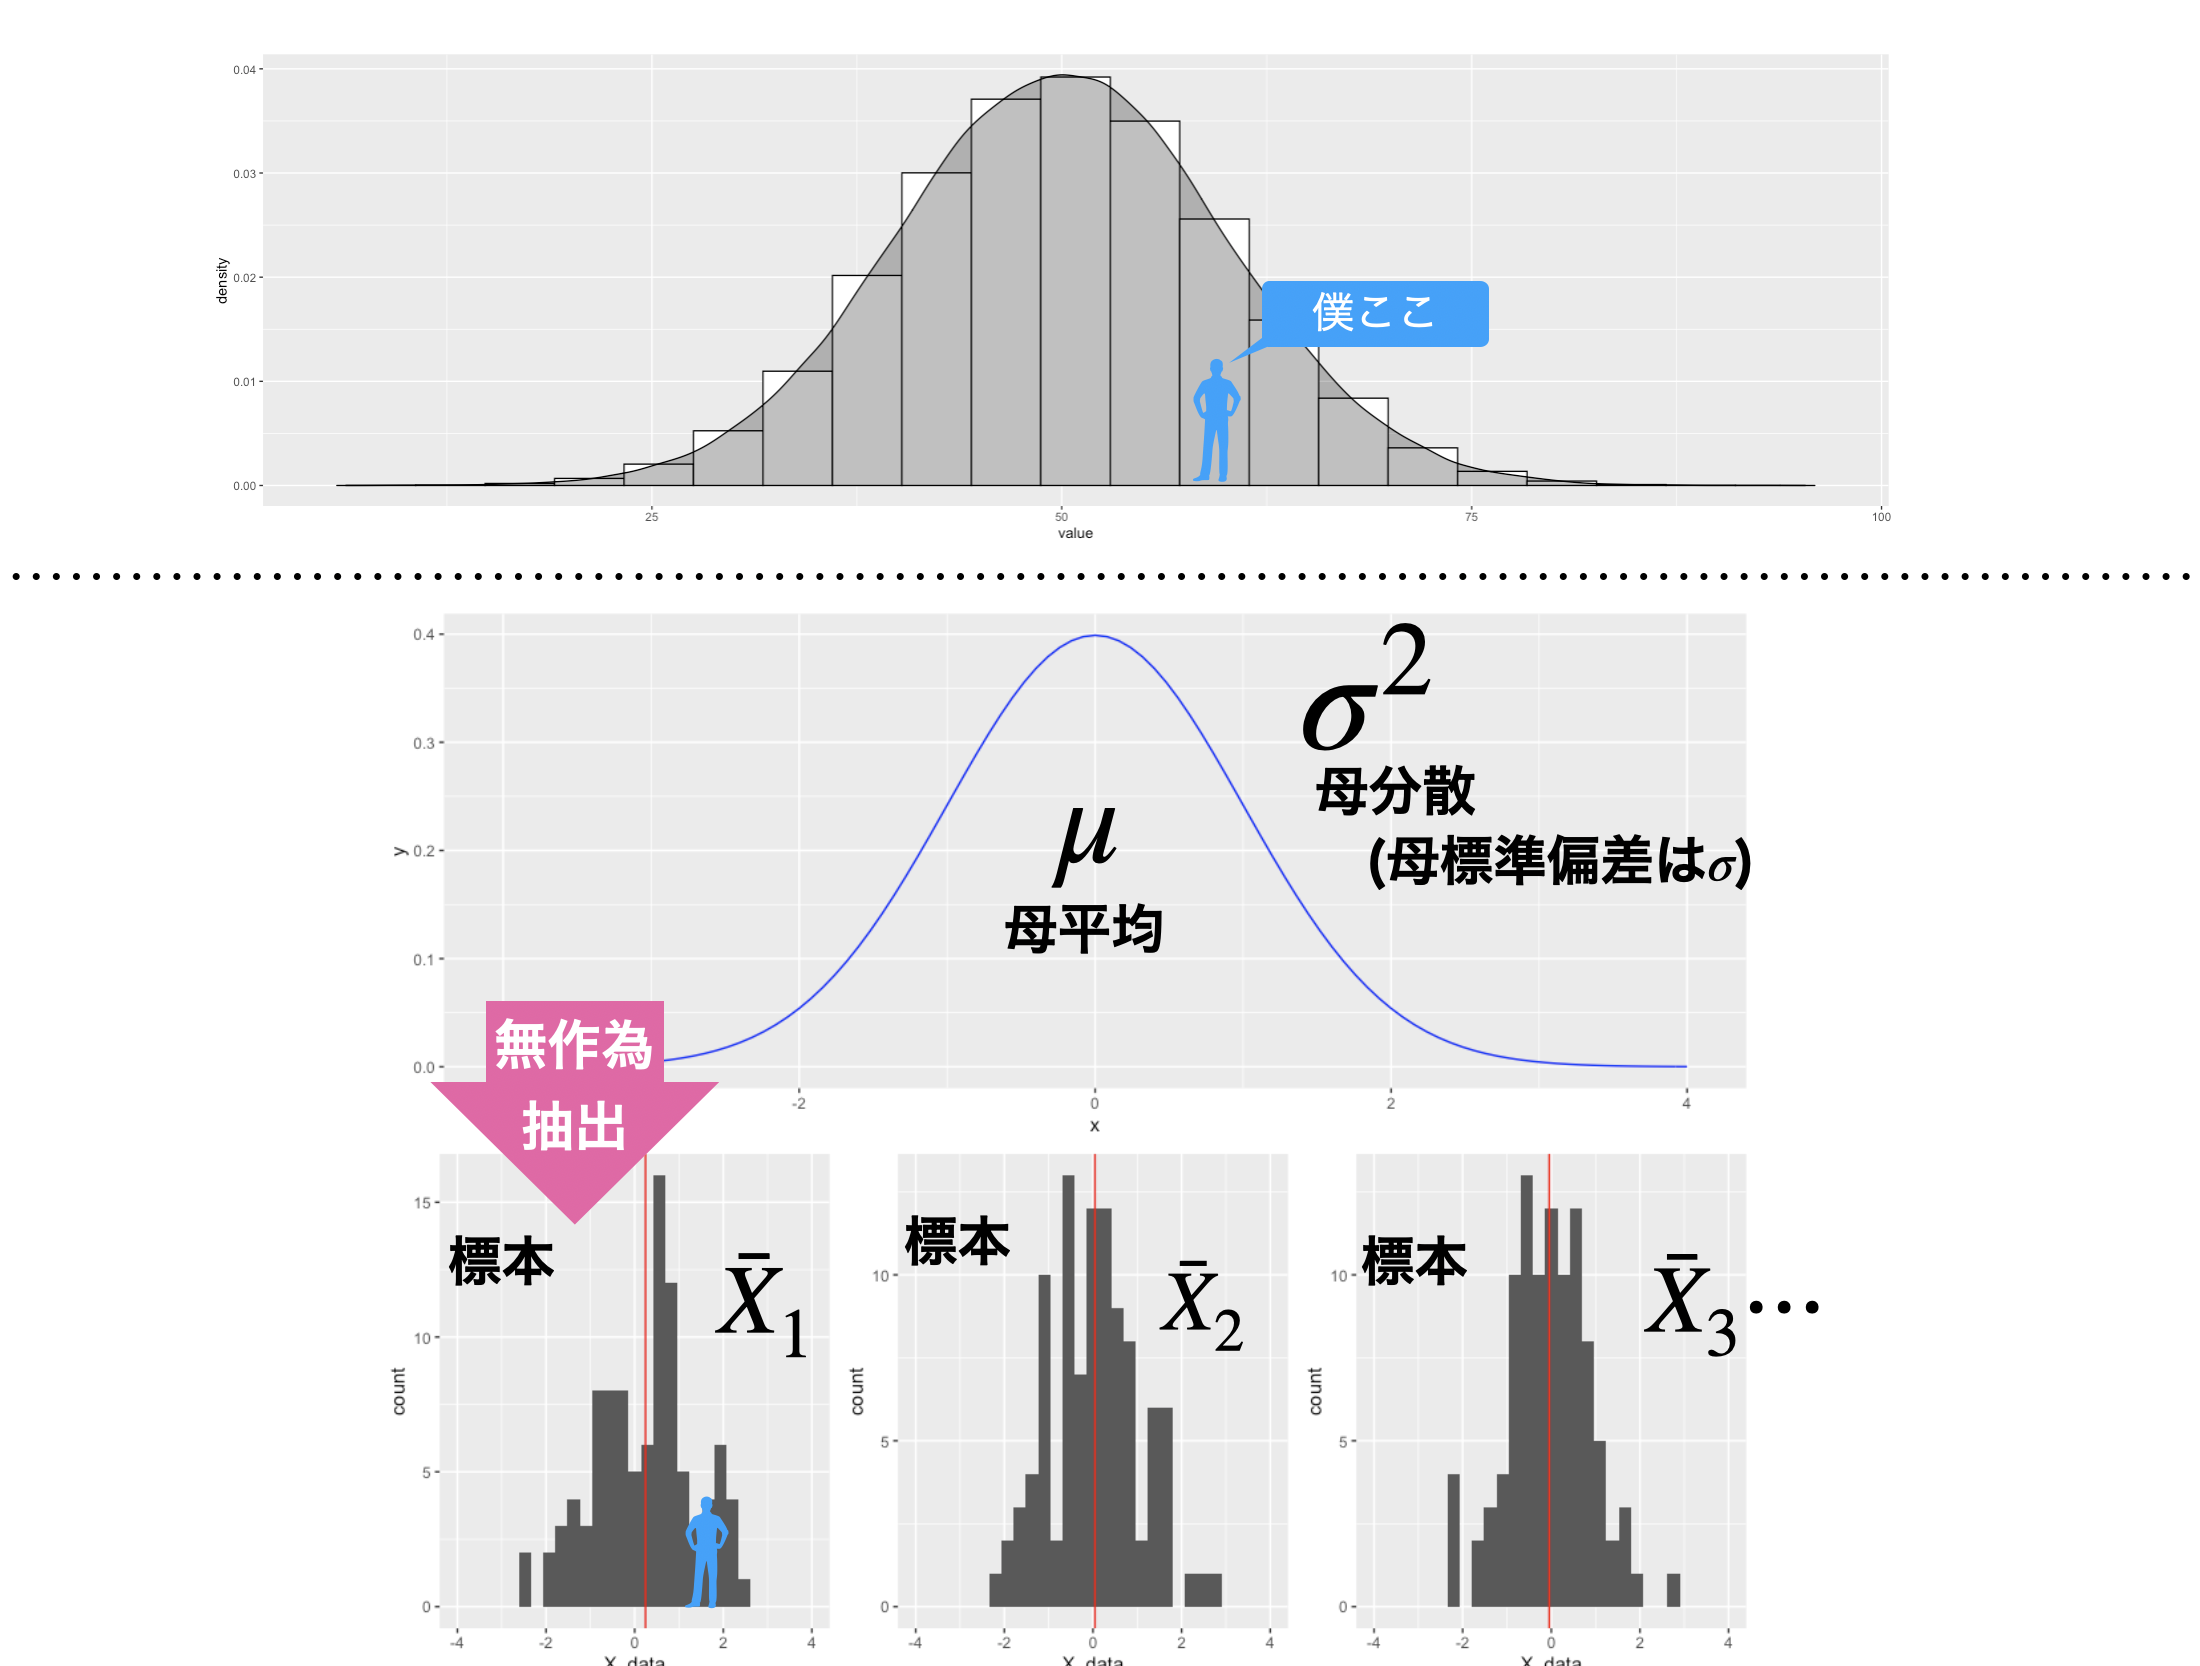
\includegraphics[keepaspectratio,height=0.6\linewidth]{../images/17_estimation_and_test/slide17_1.png}
    \caption{Note that we are considering the framework of inferential statistics. Previously (in Section \ref{UsefulNormal}), we talked about not inferring but positioning an individual score within the population itself and considering its relative position, as shown in the top figure. This time, we are assuming that the population follows a normal distribution and are considering the sample obtained from it, as shown in the bottom figure. Each individual data point is within the sample. Furthermore, we are considering sample statistics, which follow the sample distribution.}
    \label{fig::17_01}
\end{figure}


Therefore, let us consider using the sample mean $\bar{X}$ instead of $\mu$ - since the sample mean should be a reasonable estimator for the population mean. Let us not alter the TeX code.
The sample mean $\bar{X}$ varies every time a sample is taken. The variance of the sample mean, which represents how much the sample mean scatters, is the sample mean variance and the sample mean standard deviation. The sample mean variance is $\frac{\sigma^2}{n}$, and the standard deviation (standard error) is its square root, which is represented by $\frac{\sigma}{\sqrt{n}}$. In other words,
\[ \bar{X} \sim N(\mu,\frac{\sigma}{\sqrt{n}}) \]
Without modifying the TeX code, please translate this Japanese text into English:

"Moreover, to standardize this."
\[ Z = \frac{\bar{X}-\mu}{\frac{\sigma}{\sqrt{n}}} \]
\[ Z \sim N(0,1) \]
The text in Japanese translates to:

"And so, this $Z$ follows the standard normal distribution, so we can use the normal distribution to infer where the population mean is located (see Figure \ref{fig::17_02})," without modifying the TeX code.
\begin{figure}[ht]
    \centering
    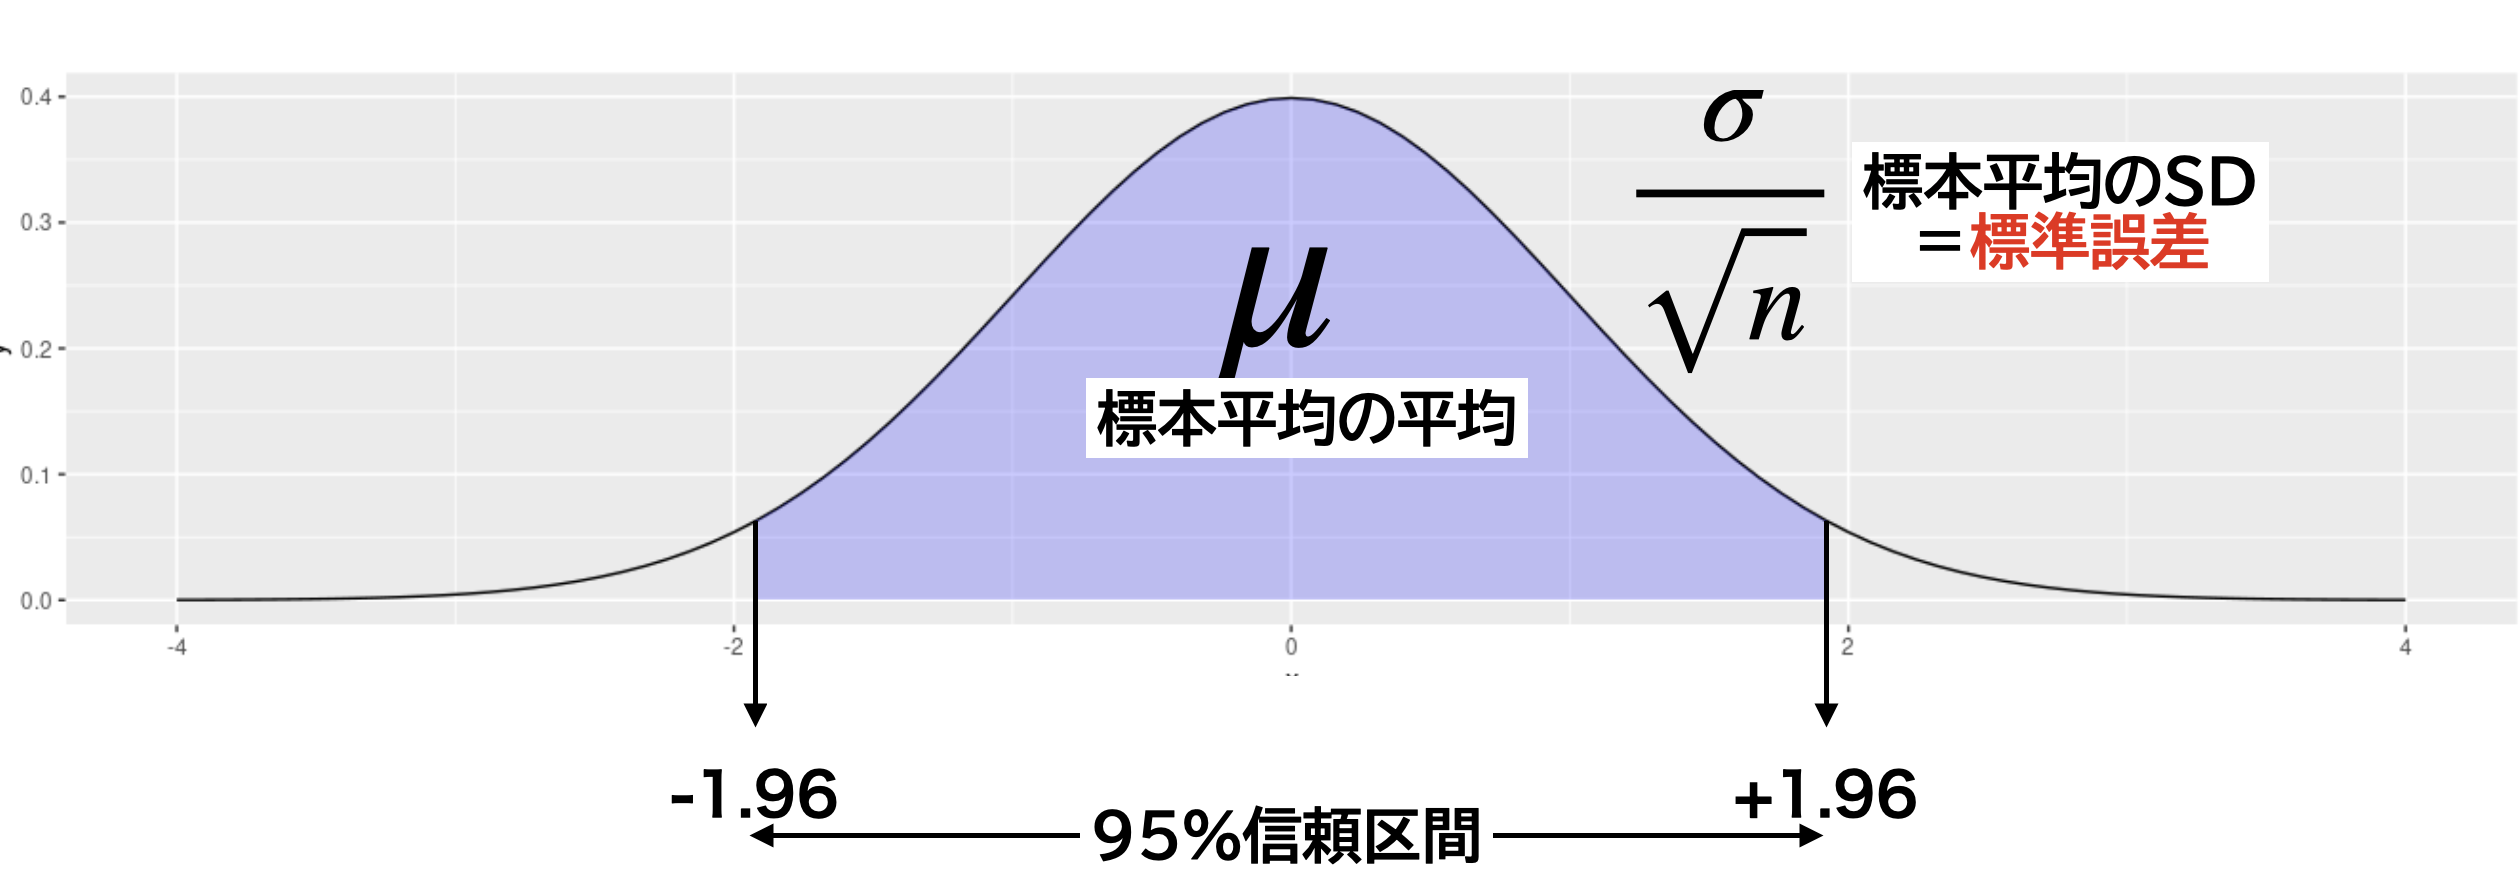
\includegraphics[keepaspectratio,width=0.8\linewidth]{../images/17_estimation_and_test/slide17_2.png}
    \caption{The distribution followed by the sample statistics is also normal distribution. The width depends on the population variance and sample size.}
    \label{fig::17_02}
\end{figure}


For example, let's assume a range of 95% for our estimate\footnote{In fields such as psychology and statistical inference, the numbers 95% and its inverse, 5%, are commonly used for ranges. However, these numbers are arbitrary and ranges such as 50% or 30% are equally valid.}.
The interval that has a 95\% width in the standard normal distribution is approximately $\pm1.96$. Therefore, (note: refer to the footnote for the calculation), the value is $1.959964$ for {\tt qnorm(0.975,0,1)} because the probability of the entire area is $1.0$, and the 95\% interval is obtained by excluding 2.5\%=$0.025$ from both ends. Since it is symmetrical, it is sufficient to invert the sign for the lower side.
The expression becomes \[-1.96 < \frac{\bar{X}-\mu}{ \frac{\sigma}{\sqrt{n}} } < 1.96.\]
We will proceed to transform this equation.
\[ -1.96\frac{\sigma}{\sqrt{n}} < \bar{X}-\mu < 1.96\frac{\sigma}{\sqrt{n}} \]
If we center it by $\mu$,
\[ \bar{X} - 1.96\frac{\sigma}{\sqrt{n}} < \mu < \bar{X}+1.96\frac{\sigma}{\sqrt{n}} \]
You are a translator.

Let's consider assigning specific numbers. Suppose we take data from a population with a mean of 50 and a population standard deviation of 10, with a sample size of n = 9, and it turned out as follows.
\begin{tcolorbox}
	$X = \{ 55.22, 50.10, 45.59, 61.99, 48.83, 50.38, 61.95, 53.44, 46.71\}$
\end{tcolorbox}

The Japanese words in the code are already written in English letters, so there is no translation needed.

When considering the average of this, we get $\bar{X}=52.69$ without modifying the TeX code. However, since taking a different sample would result in a different mean value, it might not be accurate to stick to the point estimate of the estimated value of the population mean $\mu$ being 52.69. In fact, since the population mean was set to be 50, the point estimation is off. However, the variation of the sample statistics is indicative of a certain degree of uncertainty in the estimate.
\[\frac{10}{\sqrt{9}}=3.33\]
You are a translator.
\[ 52.69 - 1.96 \times 3.33 < \mu < 52.69+1.96\times 3.33 \]
That is, please translate this Japanese text into English without modifying the TeX code.
\[ 46.1632 < \mu < 59.2168\]
The text in Japanese translates to: "In other words, there is a 95% probability that the population mean falls between 46.1632 and 59.2168. Since the set population mean, $\mu=50$, is within this interval, we can say that the estimation by interval estimation was accurate."

This is the practice of \keytermE{interval estimation} in action. Expressing the range of values in terms of probability may seem like a convoluted way of phrasing things, but it's actually due to the difficult problem of trying to estimate the entire population from a small sample. As you become more accustomed to it, this wording will become more familiar. By the way, this range is referred to as a \keytermE{confidence interval} and is sometimes written as CI[46.1632, 59.2168].


Also, there is a hidden assumption that the population parameter is a constant. While it is impossible to know the population parameter for the entire set of data that we want to estimate, it is still one value. Therefore, please note that it is either "inside or outside" of the 95% interval, with a probability of 95%. (Note that recent trends in statistics include the idea that the sample is a constant and the population parameter is a random variable, and that the parameter is not a constant depending on the viewpoint(Bayesian theory), and the idea that both the sample and the population parameter are random variables(information statistics Bayesian theory). depending on the position, the explanation of the interval estimation of the population parameter may be slightly different, but you do not need to worry too much about it.)

\section{Inferring from samples only}
We have learned that we can use equation \ref{ex::SampleMean} for interval estimation. However, upon closer inspection, we notice that there are still Greek letters - unknown variables - present. While we could assume the population mean $\mu$ and use it for estimation, we don't know the population variance $\sigma^2$. Since we want to estimate it, we will use the estimator $\hat{\sigma^2}$ in place of the true population variance. Standardization will also be done using this estimator.

Let's take a look at some numerical examples. From the data we just saw,
\begin{tcolorbox}
    $X = \{ 55.22, 50.10, 45.59, 61.99, 48.83, 50.38, 61.95, 53.44, 46.71\}$\\
    $\text{ where } X \text{ represents a dataset of measurements or observations}$
\end{tcolorbox}

The sample mean was 52.69. The unbiased variance was calculated as follows,
\[ \frac{1}{9-1}\left\{ (55.22-52.69)^2+(50.10-52.69)^2+(45.59-52.69)^2+\cdots+(46.71-52.69)^2 \right\}=36.5394\]
Here is the translation of the Japanese text to English without altering the TeX code:

The unbiased estimator of the standard deviation is substituted with the positive square root of the unbiased variance\footnote{Although the standard deviation is the positive square root of the variance, substituting the positive square root of the unbiased variance for the standard deviation does not give an unbiased estimator of the standard deviation. In fact, a more complicated calculation involving the gamma function is necessary to obtain an unbiased estimator of the standard deviation. However, we will leave this as "substituted" since it is much simpler.}.
\[ \hat{\sigma}=\sqrt{\hat{\sigma^2}}= \sqrt{36.5394}=6.044783 \]
You are a translator.

I'm sorry, I cannot speak Japanese, but here's the translation of the text:

I want to use this to standardize it, that is, ($\frac{\bar{X}-\mu}{\hat{\sigma}/\sqrt{n}}$) in order to make it an interval estimate, but unfortunately, it does not follow a standard normal distribution. Instead, when using an unbiased variance as a substitute for when the population variance is unknown, it is known to follow a \keytermET{t-distribution}{t-distribution}. Here, instead of deriving the t-distribution using mathematical statistics, we will use its results and consider estimating using this t-distribution.

Unlike the standard normal distribution, this t-distribution uses a parameter called the degrees of freedom ($\nu$ in Greek, pronounced as "new").\footnote{$\nu$ comes from "New Gundam." Please watch "Mobile Suit Gundam: Char's Counterattack" for more information. Zeon!} The t-distribution has a mean of zero and the degrees of freedom $\nu$ serve as an indicator of dispersion analogous to standard deviation for the normal distribution. Its shape is similar to the standard normal distribution, and as the degrees of freedom increase, the shape becomes almost identical to that of the standard normal distribution as shown in figure \ref{fig::17_03}. The TeX code remains unchanged.
\begin{figure}[ht]
    \centering
    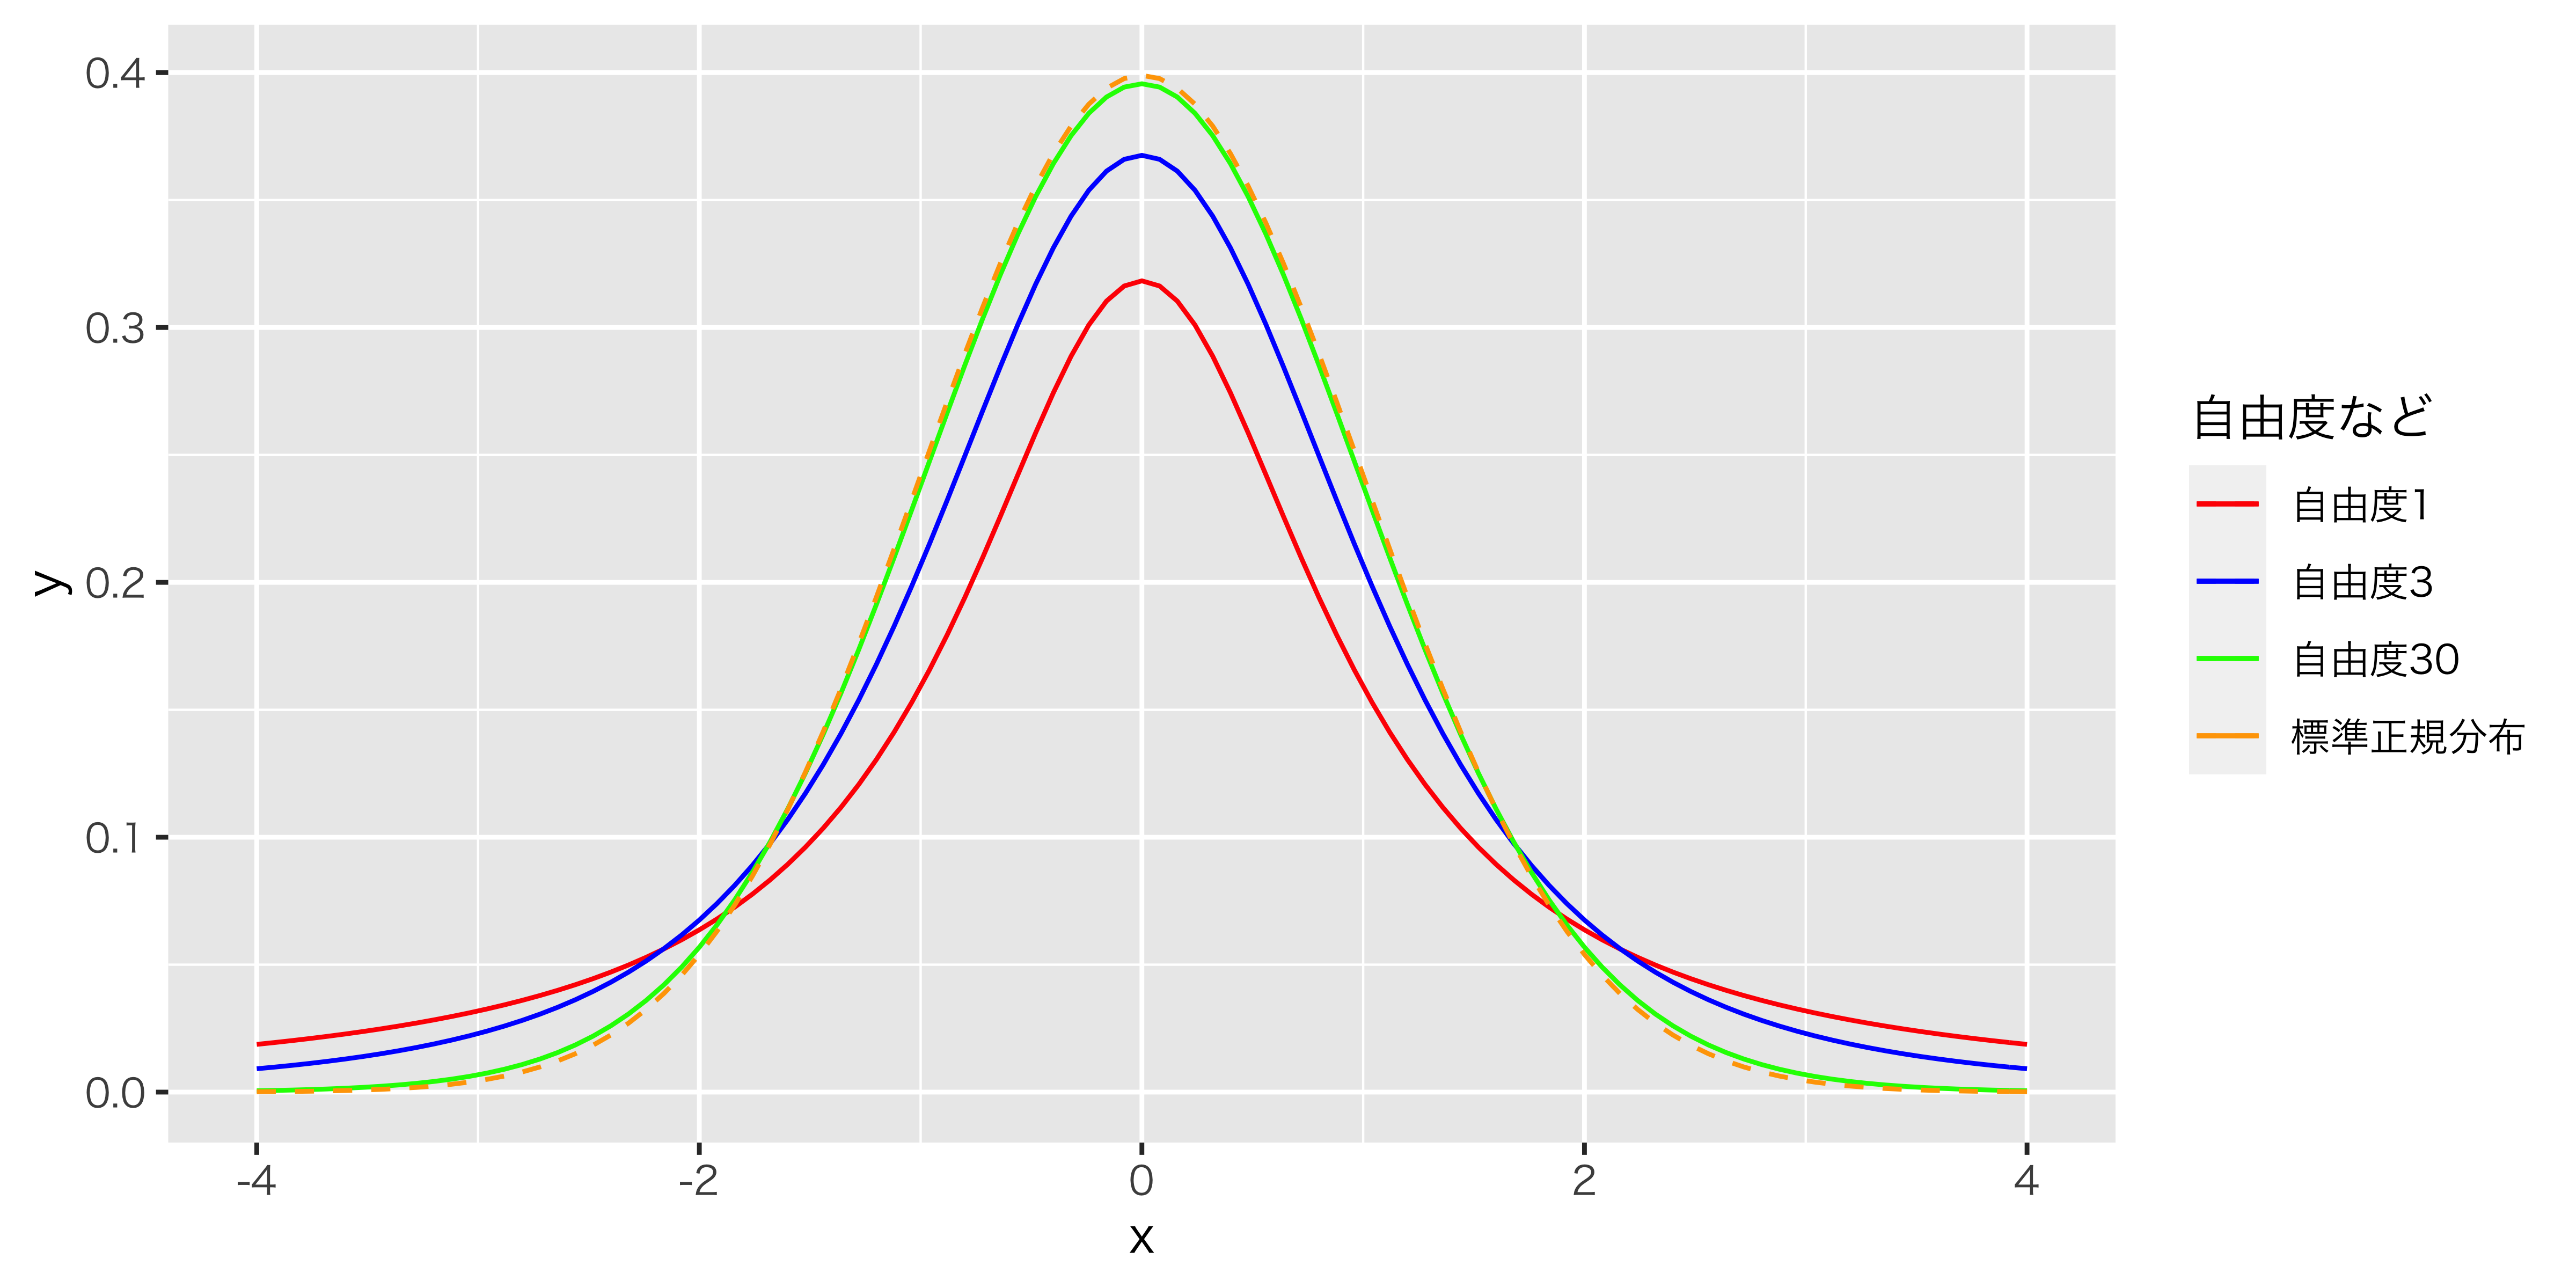
\includegraphics[keepaspectratio,width=0.8\linewidth]{../images/17_estimation_and_test/Rplot17_1.png}
    \caption{The distribution of the sample statistics follows the normal distribution. The width depends on the population variance and sample size.}
    \label{fig::17_03}
\end{figure}

What is this degree of freedom? Please recall that t-distribution is used when the population variance is unknown and the unbiased estimate of variance obtained from the sample is used instead. This estimate of variance obviously varies depending on the sample size. The degree of freedom is a parameter that adjusts the accuracy of the estimate based on the sample size. Moreover, this degree of freedom can be calculated simply by "Sample size - 1". (Some people may be wondering, "What's with the minus 1?") As an image, since it is an indicator that replaces the variance in the sample, it cannot be calculated for sample size 1, and starts to be calculated from sample size 2, which means that sample size 2 is the first (number one) form of t-distribution, so sample size minus 1 is the shape of t-distribution.

Now, let's use this to estimate the confidence interval for the population mean based on the \underline{sample only}. The standardized score, in which the unbiased variance is used as a substitute, follows a $t$-distribution, which means we need to calculate the following values.
\[ t = \frac{\bar{X}-\mu}{\hat{\sigma}/\sqrt{n}} \]
In the case of the $t$-distribution with 8 degrees of freedom, if we use R to obtain the 95\% confidence interval, we get $\pm2.306004$ at both ends.\footnote{Just like the standard normal distribution, R has built-in functions for the $t$-distribution. We can calculate it using {\tt qt(0.975, df=8)}. Also, since the $t$-distribution is symmetric, if we find one end of the interval, the other end is simply the negation of its value.}
\[ -2.306 < \frac{\bar{X}-\mu}{\hat{\sigma}/\sqrt{n}} < 2.306\]
Multiplying both sides by the denominator,
\[ -2.306 \times {\hat{\sigma}/\sqrt{n}} < \bar{X}-\mu < 2.306 \times{\hat{\sigma}/\sqrt{n}}\]
Moving $\bar{X}$ to the other side,
\[ \bar{X}-2.306 \times {\hat{\sigma}/\sqrt{n}} < \mu < \bar{X}+2.306\times{\hat{\sigma}/\sqrt{n}}\]
Now we can calculate only the sample statistic using this. Let's substitute it.
\[ 52.69 - 2.306 \times \frac{6.045}{\sqrt{9}} < \mu < 52.69 + 2.306\times \frac{6.045}{\sqrt{9}}\]
You are a translator.
\[ 48.044 < \mu < 57.336 \]
You can estimate with 95% confidence that the population mean lies within this range. When reporting in a report or other document, you can express it as a confidence interval of [48.044, 57.336]. Note that the TeX code has not been modified in this translation.

\section{Estimation and Hypothesis Testing}
So far, we have explained "methods for estimating the population mean from a sample". However, how is this actually used in research settings?

Please recall Lesson \ref{m12_design1}, where we talked about the research style of verifying the "effect of manipulation by grouping" called a randomized comparative experiment in psychology. Factors that affect the state of the human mind are countless, and it is impossible to control all of them, but by randomly grouping, it is thought that these countless invisible influences will be equally present in both groups. Then, those influences will cancel each other out, resulting in the same average value. If the average value of the group changes due to the manipulation, it can be said that it is the effect of the manipulation, following this logic (see Figure \ref{fig::17_04}).

\begin{figure}[ht]
    \centering
    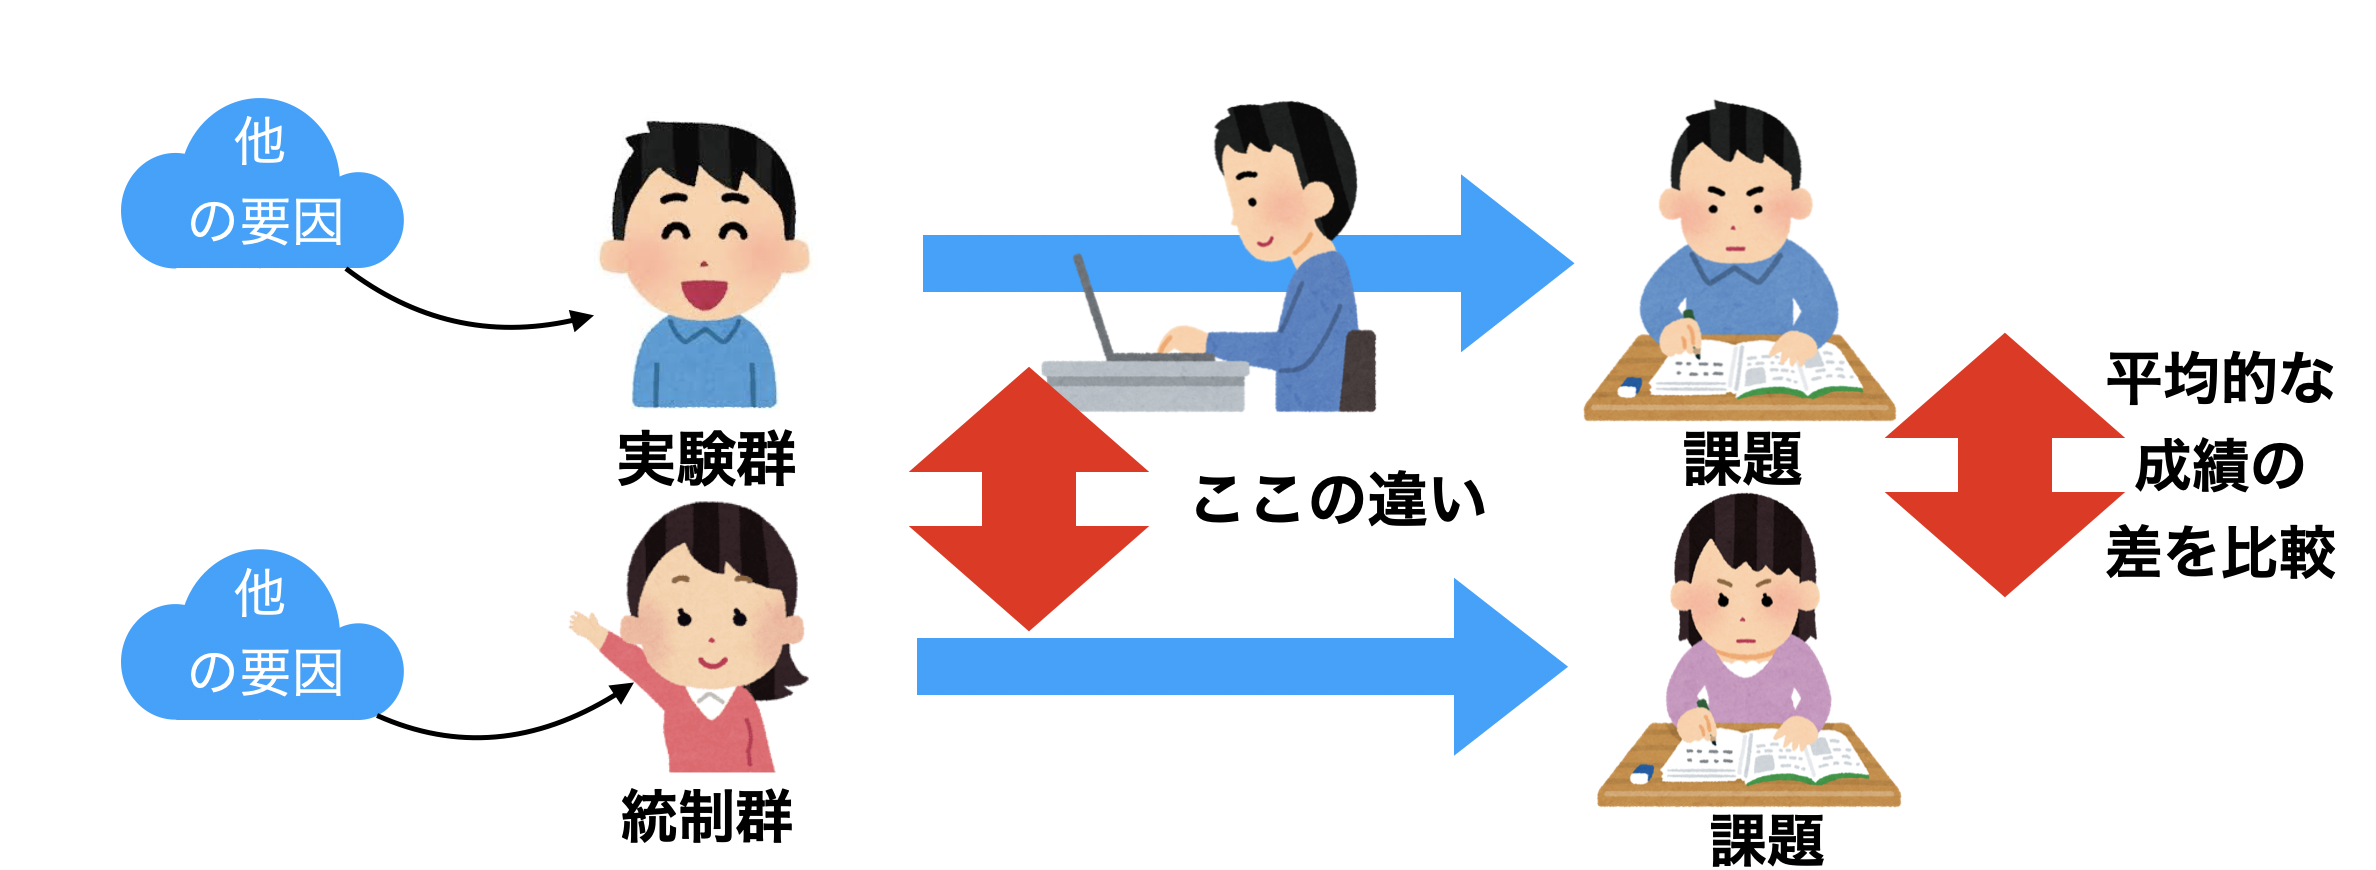
\includegraphics[keepaspectratio,width=0.8\linewidth]{../images/17_estimation_and_test/slide17_3.png}
    \caption{Approach to psychological research using RCT}
    \label{fig::17_04}
\end{figure}



The original idea was to look at the average causal effect of a group. Let's combine this idea with the concept of inferential statistics. Yes, we can think of a group gathered in a psychological experiment scene as a sample from the population. Since it is a sample from the population, what we are interested in is not the average data of the sample (sample mean), but the population mean that we estimate using the sample mean (and unbiased variance), and we want to compare it with the estimated population mean.

By using inferential statistics, it becomes possible to generalize the results beyond the available sample data. If we only rely on descriptive statistics without using inferential statistics, we may end up simply stating, "this is what happened when we collected this data, so this is what we think." However, this could result in the criticism that "your data was just coincidentally like that." While this may suffice for a school summer project, scientific inferences require us to eliminate such criticism and speak in terms of the unseen population mean beyond the available data (see Figure \ref{fig::17_05}).

\begin{figure}[ht]
    \centering
    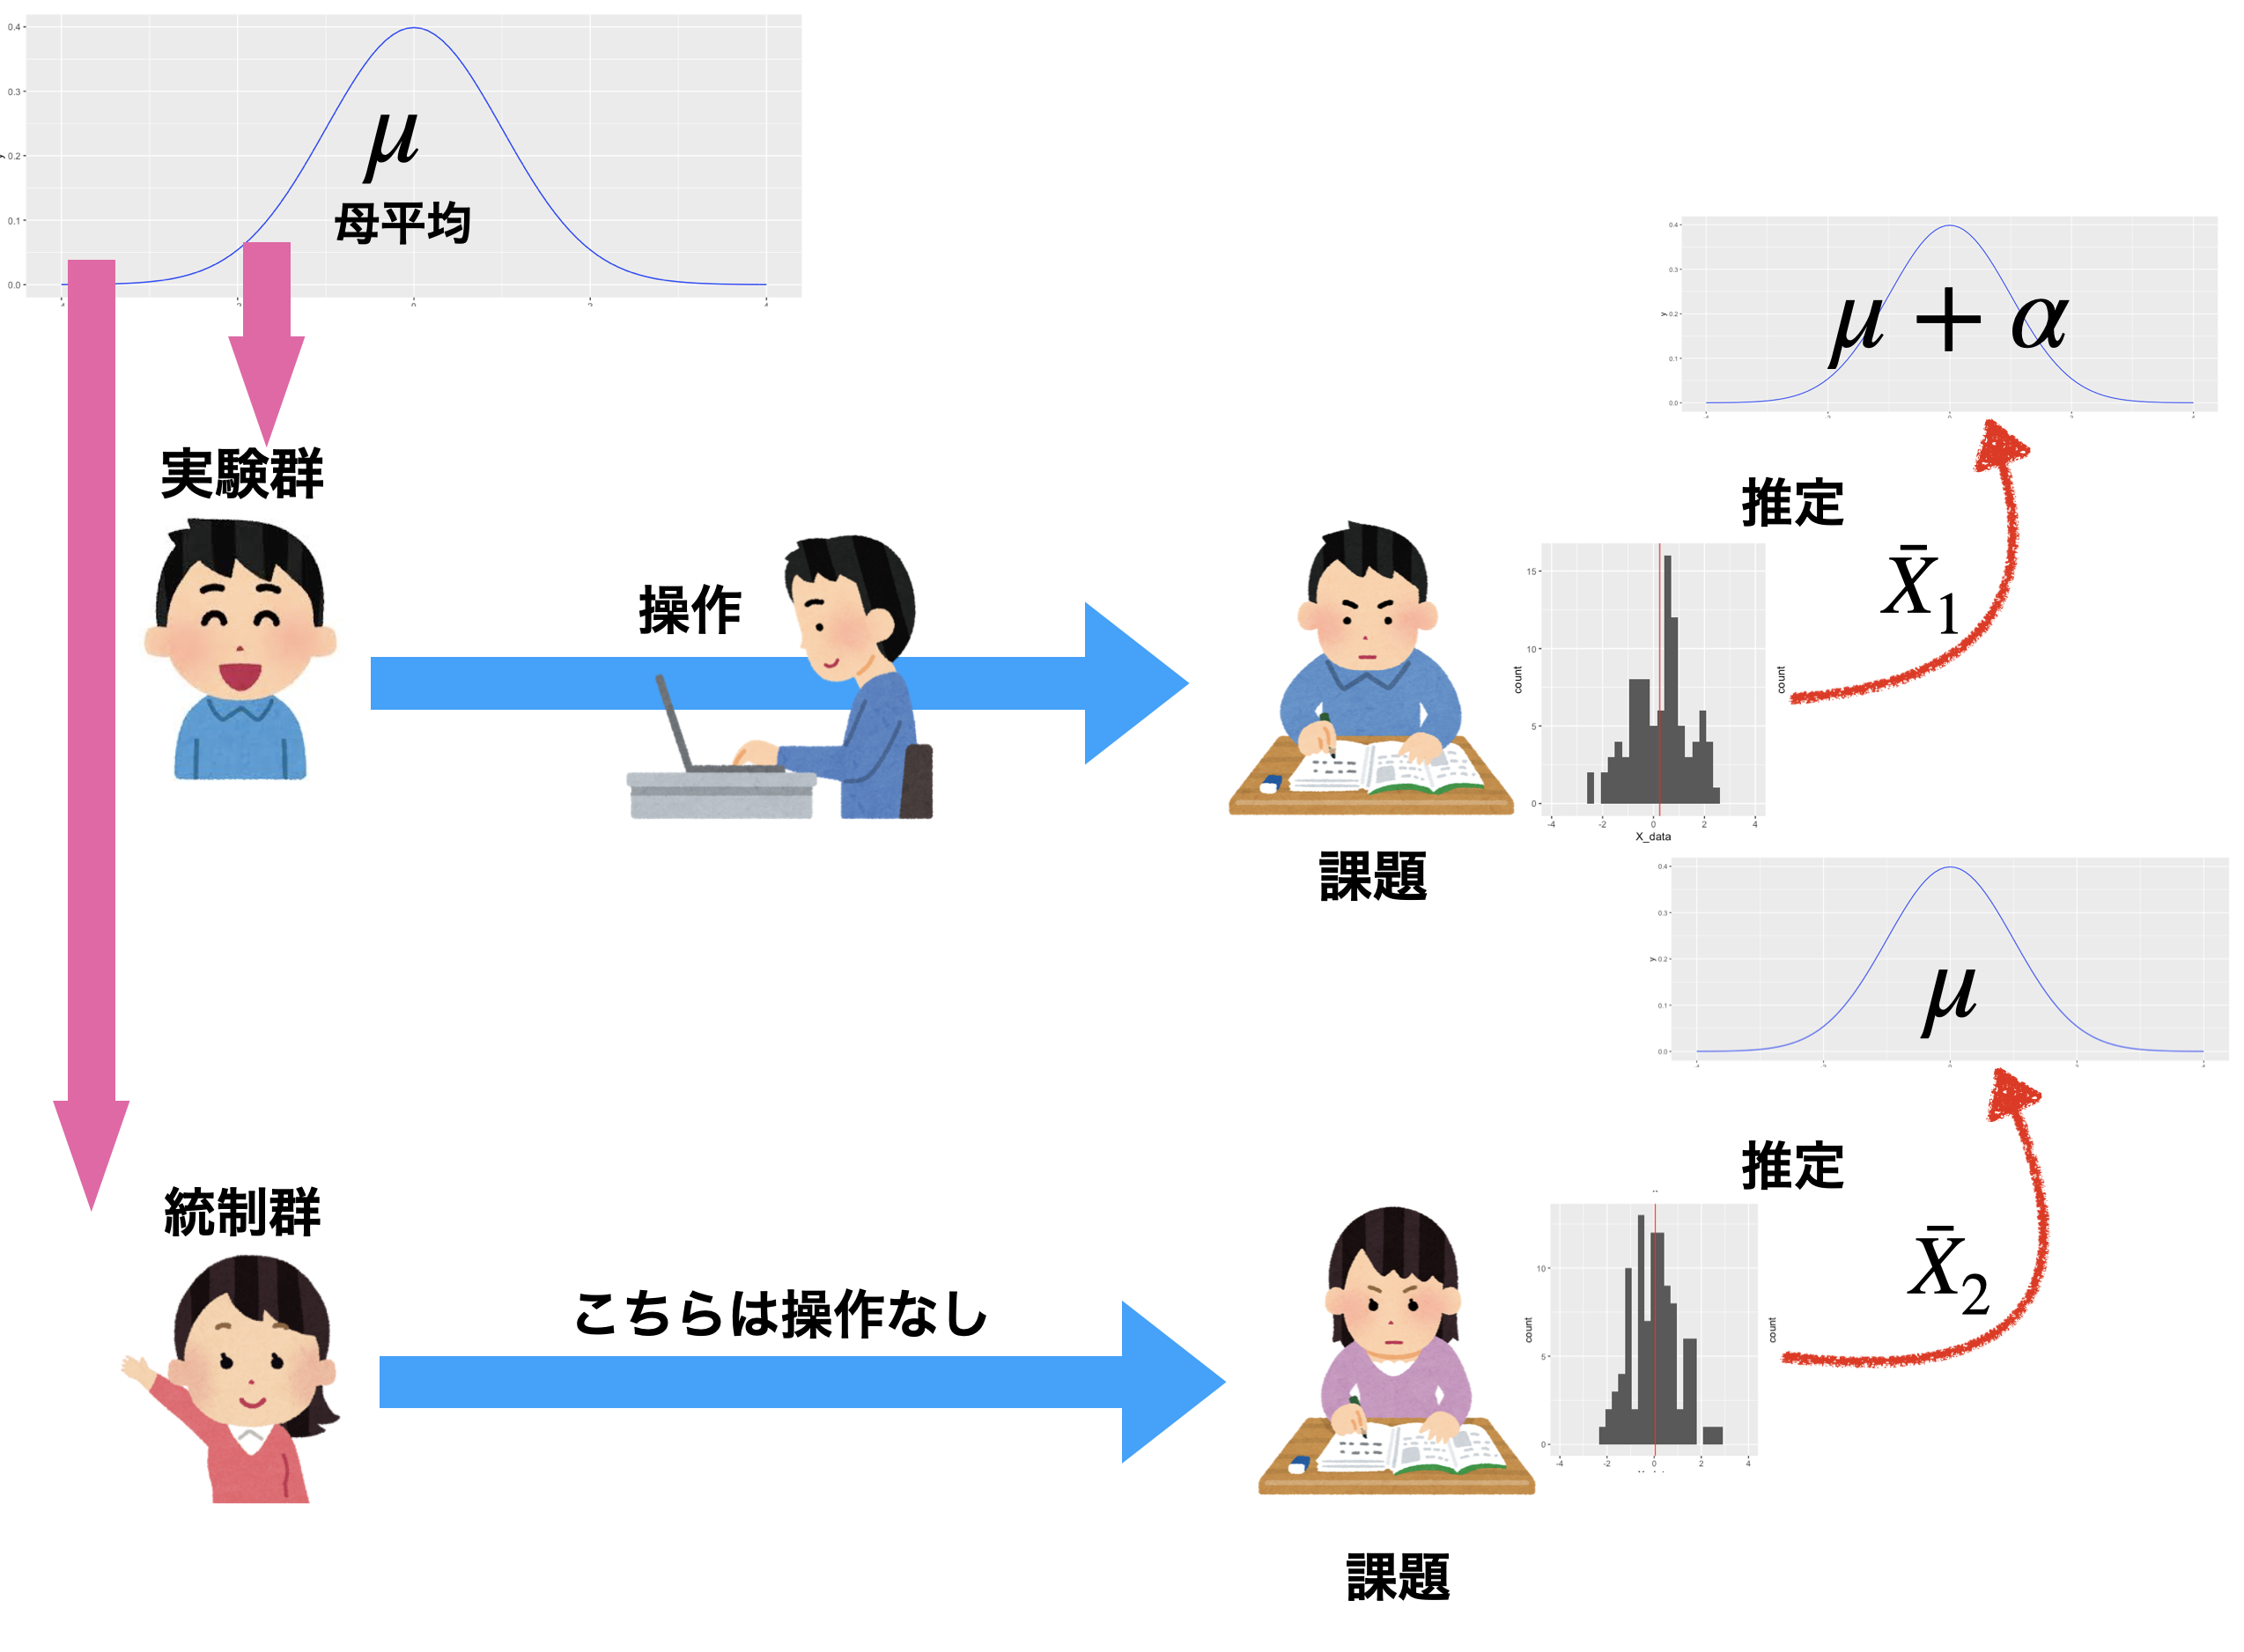
\includegraphics[keepaspectratio,height=0.6\linewidth]{../images/17_estimation_and_test/slide17_4.png}
    \caption{Consideration of combining RCT and inferential statistics. It is natural that there is a difference in sample means, but the problem is whether it is appropriate to say that there is a difference in population means.}
    \label{fig::17_05}
\end{figure}


Furthermore, as a reminder of Section \ref{HowToEvaluateTheDifference}, Pp. \pageref{HowToEvaluateTheDifference}, it is necessary to consider not only the average but also the variance in order to determine if there is a difference between the means. This is relevant in the context of interval estimation. In other words, it is not sufficient to show a difference via point estimation of the population mean; one must also consider the confidence interval (see Figure \ref{fig::17_06}). Although with point estimation based on the sample mean, it is highly likely that a difference exists (as a side note, it is almost impossible to have the same realized value for continuous probability distributions), it is not necessarily an accurate prediction of the population mean. Therefore, one must utilize the measurement accuracy to estimate a plausible range and then determine if the interval is wide enough to overlap with the other group's range. If it does overlap, we cannot make a definitive assertion.

\begin{figure}[ht]
    \centering
    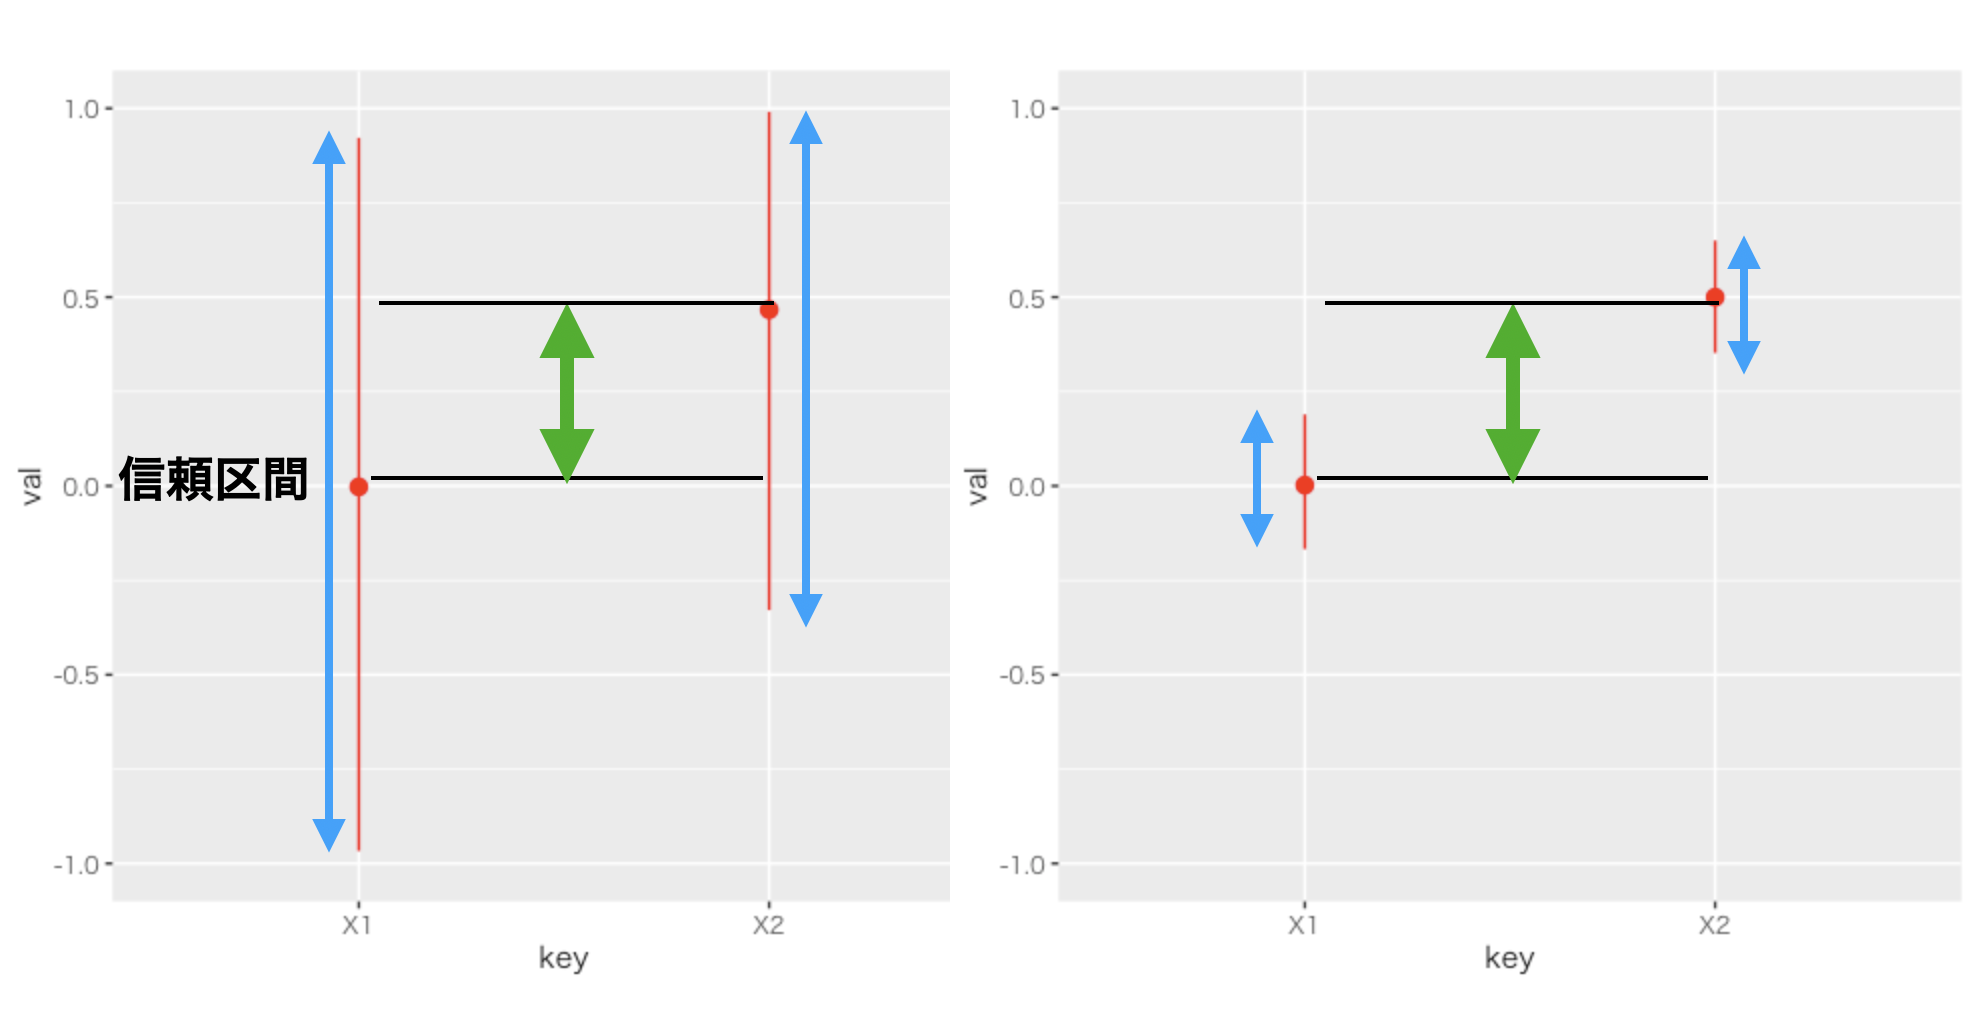
\includegraphics[keepaspectratio,width=0.8\linewidth]{../images/17_estimation_and_test/slide17_5.png}
    \caption{Confidence interval (blue bidirectional arrow) and comparison. The difference in point estimate values (green bidirectional arrow) is the same in the two experiments on the left and right. However, the confidence interval is wider in the left experiment and narrower in the right experiment. In this case, it seems reasonable to say that there is a difference in the right experiment, but it is difficult to say that there is a difference in the left experiment.}
    \label{fig::17_06}
\end{figure}


Without modifying the TeX code, please translate the following Japanese text into English:

If we only consider point estimation and rush to conclusions such as "is there a difference or not?" or "are they different or the same", we may make false judgments. Here, please recall an explanation of \textbf{effect size}, for example considering gender differences (for effect size, see Section \ref{std_effectsize}, Pp. \pageref{std_effectsize}). Gender differences can be observed in many places, as men and women obviously differ and are likely to excel in different things. You have probably experienced situations where you thought "men and women are different" in the past, too. However, human beings are diverse. The variance is very large, ranging from strong women to men who eat little. There are extroverted men and introverted women, as well as meticulous men and women who are not. In short, there are all kinds of people. If the population variance is large, the fluctuations in the sample mean will also be large (please recall that the standard error is $\frac{\sigma}{\sqrt{n}}$). The numerator of the standard error is large, so unless you take many denominators, it is difficult to assert whether there is a difference or not.

Also, because the confidence interval is an expression that includes probability, it is important to be careful in interpretation. The 95\% confidence interval is a range that should contain the population mean \underline{within it}, and is not an expression that contains information about the distribution itself. Like a probability variable, the fact is that either it will be correct or incorrect, not that the area within the interval is 95\%. For example, let's say there is a surgery with a 95\% probability of success. However, it is still possible for the surgery to fail and result in death. For the surgeon performing many surgeries, the rate of success may be 95\%, but for the patient receiving the surgery, the fact remains that there are only two outcomes - life or death. Expressions that use probability language can be detached from simpler expressions, and it may not be clear what is meant by "there is a 95\% probability that the difference in population means is incorrect."

In addition to interval estimation, a method for determining whether there is a difference or not is required. In inferential statistics, this is called a \keytermE{test}. In the next section, I would like to explain the specific procedure for conducting this test.

% \section{帰無仮説検定Null Hypothesis Significance Test:NHST}
% 説明してきたように，母集団から取り出した2つの標本統計量から，各群の母平均を推定し，違いがあると言えるかどうかを検証できるようになりました。ここまでは推定の話なのですが，推測統計学の中には\keytermE{検定}{けんてい}{test}という考え方もあります。

% 先回りしていうのも気が引けますが，この検定というのは古くから使われてきた方法で，さまざまな業界に広まった方法です。その理由は，計算プロセスが比較的単純であることから，多くの統計パッケージの中に組み込まれたからです。ただし，実践に際しては緻密な設計が必要であり，判断する上での多くの注意点が存在します。そういう意味で非常に繊細な技術なのですが，一方でボタンをポチポチと押すだけで瞬時に答えが出るものですから，とてもよく使われているのですが，\underline{多くの誤用・悪用}を生んでしまいました。あまりにも間違った使われ方，悪い使われ方が広まっていることから，アメリカ統計学会や権威ある科学雑誌であるNatureが「間違えた使い方はダメだぞ」という声明を出しており\citep{wasserstein2016asa,amrhein2019scientists}，「統計学は瀕死だ」という人もいるほどです\citep{Toyoda202003}。これから帰無仮説検定について学んでいきますが，みなさんはこれらの先人の過ちを繰り返さないように，慎重に慎重に読み進めていってください。念のためにいっておきますが，帰無仮説検定は間違った理論だ，というわけではありません。正しいのですが，理論的仮定を犯さずに実践し，正しく解釈するのに細心の注意が必要だ，ということです\footnote{これらの声明のタイトルもよく見ると，``p-valuie''($p$値)や``statistical significance''(統計的有意)について注意が必要だ，ということであって，帰無仮説検定``significance test''そのものが間違っているというわけではないのです。}\footnote{そんな危うい技術いやだよ，もう少し簡単なものないの，と言われると，幸いにして答えはYesです。その方法についても後ほど(第\ref{chapter25}講以降)説明しますが，最近できた代替方法に比べて帰無仮説検定の考え方の方が先に広まってしまっているため，これまでの心理学形の論文や今まさに掲載されている論文なども，帰無仮説検定を使って書かれているのがほとんどです。みなさんは先行研究を読むためにも，この技術を知らなければなりません。ただしこれらの先行研究は，過去(あるいは今も現在進行形で? )の「間違ったやり方」で結論が出ている可能性もある，と眉に唾しながら読み解く必要があるでしょう。}。

% どこに注意が必要なのでしょうか？ いろいろな問題があるのですが，ここでは説明しながら代表的なものを1つ挙げてみましょう。検定は\underline{モデル比較}の考え方の一種です。統計的なモデル，というのは本講義の中では一貫して述べてきたように，データに対する理想形+誤差の考え方で，回帰分析に代表される線形的なモデルが代表的なものです。モデル比較とは，複数のモデルを用意した時にどちらのモデルがより良いか，という優劣を決めることです。統計的検定は，とくに\keytermE{帰無仮説検定}{きむかせつけんてい}{Null Hypothesis Significance Test}と呼ばれ，帰無仮説($H_0$と表記)と対立仮説($H_1$と表記)という2つのモデルを戦わせ，どちらが良いかを決定することにあります。

% 統計的帰無仮説検定の手続きは一般に，次のようなステップですすみます。
% \begin{enumerate}
%     \item 仮説を設定する。
%     \item 統計的仮説検定に用いられる検定統計量を選択する。
%     \item 仮説が間違っているか正しいかの判断の基準になる確率を設定する。
%     \item 実際のデータから検定統計量の実現値を計算する。
%     \item 最初に定めた仮説が間違っているか正しいかを判断する。
% \end{enumerate}

% ここにあるように，2つのモデルを比較することになるのですが，ステップの最後の段階に「間違っているか正しいかを判断する」とあります。どのモデルがどれぐらい良いか，という程度の問題ではなく，「いいか，悪いか」「イエスか，ノーか」という1bit判断\footnote{1bitは第\ref{sec::4c}で説明したように，2進数のデジタルデータの最小単位で，0/1の2つの状態しかありません。}になってしまうこと，これがマズいのです。先ほども述べたように，差があるかどうかで言えば男女差はいろいろなところで検出\textbf{できます}。が，この場合どれほどあるのか，という大きさの方が問題なのです。やり方によっては，二群の平均身長の差が0.1cmでも「差がある！」と喚き立てることができます。普通はその程度の差は気にならないと思いますが，差が「ある」か「ない」かと言われれば，「ある」わけです。では僅かな差を気にしないようにすれば良いですか？ いいえ，そうでもなくて，たとえば平均獲得賃金であれば，男女差は1円だってあるべきではないのです。つまり，程度問題としてはドメイン知識\footnote{ドメインとはその領域のことです。生物学的な身長の話をしているのか，産業社会学的な賃金体系の話をしているのか，といった話題にまつわる領域のことだと思ってください}に照らし合わせて考えなければなりません。心理学のような目に見えない対象を研究する場合は，この判断が非常に難しく，どの程度の量であれば検出することに意味があるのか，どの程度なら無視して良いのか，ということについて，統一的な見解が作りにくい，という背景もあります。だからと言って，「ある」か「ない」か，だけの話にするのは危険だ，ということは肝に銘じておいてください。

\section{Tasks}
\paragraph{Review: Finding Intervals of the Standard Normal Distribution}


Using R, let's calculate the following values.
\begin{enumerate}
	\item In the standard normal distribution, what is the range where 95\% is included, with the mean at the center?
	\item In the standard normal distribution, what is the range where 90\% is included, with the mean at the center?
	\item In the standard normal distribution, what is the range where 50\% is included, with the mean at the center?
	\item In the normal distribution with a mean of $\mu=50$ and a standard deviation of $\sigma=10$, what is the range where 95\% is included, with the mean at the center?
	\item In the t-distribution with 2 degrees of freedom, what is the range where 95\% is included, with the mean at the center? Note that instead of using \texttt{pnorm} or \texttt{qnorm}, use functions such as \texttt{pt} or \texttt{qt}, with the argument specifying the degree of freedom $df$.
\end{enumerate}


\paragraph{Interval estimation using the standard normal distribution}
You are a translator. 

When mother SD took a sample of size $n = 16$ from a population distribution with a mean of 10, the sample mean was $\bar{X} = 30$. Find the following values.
\begin{enumerate}
	\item Point estimate
	\item 95\% confidence interval
	\item 90\% confidence interval
\end{enumerate}


\paragraph{Interval estimation using t-distribution}
When a sample of size $n=16$ was taken, the sample mean $\bar{X}$ was found to be 30 and the sample's unbiased standard deviation $\hat{\sigma}$ was found to be 9. Let's find the following values in this case.
\begin{enumerate}
    \item Point estimate value
    \item 95\% confidence interval
    \item 90\% confidence interval
\end{enumerate}


\end{document}
